%------------------------------------------------------------------------------
% Manuscript for Acta Crystallographica Section A, prepared with the IUCr
% LaTeX macro package (iucr.cls).  Compile with pdflatex.
%------------------------------------------------------------------------------
\documentclass[preprint,pdf]{iucr}          % DO NOT DELETE THIS LINE
\journalcode{A}

\usepackage{amsmath,amssymb}
\usepackage{booktabs}
\usepackage{array}
\usepackage{graphicx}

\newcommand{\Ang}{\text{\AA}}
\newcommand{\Gmet}{\mathbf{G}}
\newcommand{\Pop}{\mathbf{P}}
\newcommand{\Wop}{\mathbf{W}}
\newcommand{\Sw}{\mathcal{S}_\tau}
\newcommand{\Se}{\mathcal{S}_\epsilon}
\newcommand{\Cl}{\mathcal{C}}
\newcommand{\Laue}{\mathcal{L}}
\newcommand{\Lay}{\mathcal{N}}
\newcommand{\sym}{\operatorname{sym}}
% every checkable statement carries \chk{zNN}: the test file
% manuscript/appendix_z/test_zNN_*.py that verifies it (Appendix E)
\newcommand{\chk}[1]{\textsuperscript{[#1]}}

\begin{document}                  % DO NOT DELETE THIS LINE

\title{The Selling closure: complete reindexing of measured lattices}
\shorttitle{The Selling closure}

\cauthor{Petrus H.}{Zwart}{phzwart@lbl.gov}{}
\aff{Molecular Biophysics and Integrated Bioimaging Division, Lawrence Berkeley National Laboratory, 1 Cyclotron Road, Berkeley, CA 94720, \country{USA}}
\shortauthor{Zwart}

\keyword{Selling reduction}\keyword{obtuse superbase}\keyword{Delone sorts}\keyword{lattice symmetry}\keyword{reindexing}\keyword{pseudo-symmetry}\keyword{groupoid}

\maketitle                        % DO NOT DELETE THIS LINE

\begin{synopsis}
All reduced cells of a lattice and the integer matrices between them form a finite, complete groupoid. Widened in a strain norm that is the same in every basis, it is computed exactly for measured cells and turns reindexing into a lookup.
\end{synopsis}

\begin{abstract}
A lattice with a right angle has several Selling-reduced cells, related by integer matrices that are symmetries of nothing. We treat the set of all obtuse superbases of a lattice, with the unimodular matrices between them, as one object, the Selling closure. It is a finite groupoid: the matrices from a cell to itself form the lattice point group, those between cells are the alternative reduced settings, and the matrices between any two settings form a coset of the point group. The closure is complete and is generated from any member by a fixed set of 6096 integer matrices. For a measured cell it is widened to every superbase within a strain $\epsilon$ of obtuse, in the affine-invariant norm on metric tensors, which is the same in every basis. The widened set is finite and is enumerated exactly; filtering a fixed layer of operators is proved exact up to an adjacency radius computed for each cell, which exceeds Le Page's $3^\circ$ for cells of ordinary shape, and a second layer covers needles and plates. Reindexing a new cell onto a reference then needs one reduction of the new cell: the candidates form one coset, and its classes under the Laue group are the distinct indexings, each with a strain price. On 780 constructed cases the true operator was among the candidates in every case.
\end{abstract}

%==============================================================================
\section{Introduction}
%==============================================================================

Two questions recur in indexing and data processing: what are the symmetries of a lattice, and are two cells the same lattice, and if so by which integer matrix? Both are usually answered by searching. Symmetry is found by scanning for near-twofolds within an angular tolerance (Le Page, 1982; Sauter \emph{et al.}, 2004); reindexing tries a list of small integer matrices, or the operators of the point group just found. The symmetry search is complete within its index bound. The reindexing search is complete only if the list happens to contain the operator. Both are complicated by the same fact: a lattice with a right angle has more than one reduced cell, and the alternatives are related by integer matrices that are not symmetries.

Selling reduction makes this multiplicity explicit. A superbase is four lattice vectors summing to zero; it is obtuse, or Selling-reduced, when all six pairwise dot products are non-positive (Selling, 1874). A superbase is obtuse exactly when its partial sums are the Voronoi vectors of the lattice (Voronoi, 1908; Conway \& Sloane, 1992), the obtuse superbase is unique except when a dot product vanishes (Delaunay, 1933; Patterson \& Love, 1957), and Kurlin (2022) listed all obtuse superbases of each zero pattern and showed that their six values form a complete isometry invariant of the lattice, the root invariant. Delaunay's 24 sorts classify lattices by the zeros and equalities among those values (Delone \emph{et al.}, 1975; Burzlaff \& Zimmermann, 2006; Andrews \& Bernstein, 2023\emph{b}). The same objects appear as $S^6$ with its boundary transformations (Andrews \emph{et al.}, 2019\emph{a},\emph{b}) and in SELLA (Andrews \emph{et al.}, 2023). On the Niggli side, the multiplicity of Buerger cells (Buerger, 1960; Gruber, 1973) and the instability of the reduced cell under error (Andrews \emph{et al.}, 1980; Andrews \& Bernstein, 1988) are the same phenomenon. For measured cells, distances to Bravais-lattice subspaces are measured by Andrews \& Bernstein (2014) and by Oishi-Tomiyasu (2012, 2024), whose error-stable Bravais-lattice determination comes with a bound under which a finite list of basis transforms is provably enough; the operators relating two settings form a coset of the symmetries (Flack, 1987).

This paper takes the whole set of obtuse superbases of a lattice, with the integer matrices between them, as the object of study. We call it the \emph{Selling closure}. What is added to the classical material is:
\begin{enumerate}
\item the closure as a finite, complete groupoid, holding the point group and every alternative reduced setting, and its computation for all 24 sorts from integer matrices alone;
\item for a measured cell, the widened closure in a strain norm that is the same in every basis, a finite set that is enumerated exactly;
\item a layered computation of it, proved exact up to a radius computed for each cell, in tiers: the first layer for cells of ordinary shape, a second layer or a finite ball for needles and plates;
\item reindexing from one reduced cell of the new measurement, with the candidates forming one coset whose classes under the Laue group are the distinct indexings.
\end{enumerate}

Section~\ref{sec:background} collects the classical definitions. Section~\ref{sec:closure} defines the closure as a groupoid and works through one monoclinic cell. Section~\ref{sec:measured} states the computations for measured cells. Section~\ref{sec:results} gives the closures of the 24 sorts, the distances of measured cells to the sorts, the completeness of the computation and the reindexing results. Proofs are in Appendix~A; the special case of a band on the conorms, the first version of this work, in Appendix~B; catalogues in Appendix~C; the operators with no lattice in Appendix~D. Every computed number carries a mark [z$nn$] naming the check that reproduces it (Appendix~E).

%==============================================================================
\section{Background}
\label{sec:background}
%==============================================================================

\subsection{Superbases, conorms and the metric tensor}
\label{sec:defs}
Selling reduction works with four vectors: the cell vectors $a$, $b$, $c$ and $d=-a-b-c$. The four form a \emph{superbase}; any three of them are a basis of the lattice. The six negated pair products
\[
p_{da}=-d\cdot a,\quad p_{db}=-d\cdot b,\quad p_{dc}=-d\cdot c,\quad p_{ab}=-a\cdot b,\quad p_{ac}=-a\cdot c,\quad p_{bc}=-b\cdot c
\]
are the \emph{conorms} (Selling, 1874; Conway \& Sloane, 1992); the Selling parameters of $S^6$ (Andrews \emph{et al.}, 2019\emph{a},\emph{b}) are the same numbers with the opposite sign. Conorm vectors are written in the slot order $da,db,dc,ab,ac,bc$, except that the sort patterns of Table~\ref{tab:sorts} use the $S^6$ order $bc,ac,ab,ad,bd,cd$ for comparison with Andrews \& Bernstein (2023\emph{b}). A superbase is \emph{obtuse}, which is to say Selling-reduced, when all six conorms are non-negative. The metric tensor in the basis $(a,b,c)$ is linear in the conorms,
\begin{equation}
\Gmet=\begin{pmatrix}
p_{ab}+p_{ac}+p_{ad} & -p_{ab} & -p_{ac}\\
-p_{ab} & p_{ab}+p_{bc}+p_{bd} & -p_{bc}\\
-p_{ac} & -p_{bc} & p_{ac}+p_{bc}+p_{cd}
\end{pmatrix},
\label{eq:gram}
\end{equation}
so the conorms are six cell parameters. A zero conorm is a right angle between two of the four vectors; the set of slots that vanish is the \emph{zero pattern}. If the non-zero conorms are to connect the four vectors, there are five kinds of zero pattern up to relabelling, which correspond to the five types of Voronoi polyhedron (Voronoi, 1908; Conway \& Sloane, 1992); with the two placements of three zeros (a triangle or a path) there are 38 faces of the cone of non-negative conorms, a face being where a chosen set of conorms vanishes.

\subsection{Flips and swaps}
\label{sec:operators}
Two kinds of integer operator act on a superbase.

\emph{Flips.} A flip at the conorm $p_{ab}$ replaces $a$ by $-a$ and adds the old $a$ to the two other vectors, $(a,b,c,d)\mapsto(-a,\ b,\ c+a,\ d+a)$. The new conorms are $p'_{ab}=-p_{ab}$, $p'_{ac}=p_{ad}+p_{ab}$, $p'_{da}=p_{ac}+p_{ab}$, $p'_{bc}=p_{bc}+p_{ab}$, $p'_{db}=p_{db}+p_{ab}$ and $p'_{dc}=p_{dc}-p_{ab}$; this is the boundary transformation of Andrews \emph{et al.} (2019\emph{a}), written on the basis. Selling reduction applies flips at negative conorms until none remain. When $p_{ab}$ is exactly zero the flip exchanges the slots $ac$ and $da$ and carries one obtuse superbase to another of the same lattice, which is why the reduced cell of a lattice with a right angle is not unique; all reduced cells of a lattice carry the same six conorm values, the root invariant of Kurlin (2022). In the basis $(a,b,c)$ each flip is a fixed $3\times3$ integer matrix of determinant $-1$ that is its own inverse (Table~\ref{tab:flips}). A word of flips such as $ab.bc.db$ is applied left to right, each flip read in the current labelling, and its matrix is $\mathbf F_{ab}\mathbf F_{bc}\mathbf F_{db}$, columns being the new basis vectors in the old basis.

\begin{table}
\caption{The six Selling flips as $3\times3$ integer matrices in the basis $(a,b,c)$, $d=-a-b-c$; columns are the new basis vectors in the old basis. Each has determinant $-1$ and squares to the identity. For the flips at $da$, $db$, $dc$ the vector $d$ is negated and the new $a,b,c$ are listed.}
\label{tab:flips}
\begin{tabular}{lll}
\toprule
flip at & new basis & matrix \\
\midrule
$ab$ & $(-a,\ b,\ a+c)$ & $\begin{pmatrix}-1&0&1\\0&1&0\\0&0&1\end{pmatrix}$ \\[1.5ex]
$ac$ & $(-a,\ a+b,\ c)$ & $\begin{pmatrix}-1&1&0\\0&1&0\\0&0&1\end{pmatrix}$ \\[1.5ex]
$bc$ & $(a+b,\ -b,\ c)$ & $\begin{pmatrix}1&0&0\\1&-1&0\\0&0&1\end{pmatrix}$ \\[1.5ex]
$da$ & $(a,\ -a-c,\ -a-b)$ & $\begin{pmatrix}1&-1&-1\\0&0&-1\\0&-1&0\end{pmatrix}$ \\[1.5ex]
$db$ & $(-b-c,\ b,\ -a-b)$ & $\begin{pmatrix}0&0&-1\\-1&1&-1\\-1&0&0\end{pmatrix}$ \\[1.5ex]
$dc$ & $(-b-c,\ -a-c,\ c)$ & $\begin{pmatrix}0&-1&0\\-1&0&0\\-1&-1&1\end{pmatrix}$ \\
\bottomrule
\end{tabular}
\end{table}

\emph{Swaps.} A superbase is an unordered set of four vectors up to a common sign, so one reduced cell can be written in $4!\times2=48$ ways. The 48 reorderings and sign changes are the swaps; they change which vectors are called $a,b,c$ and nothing else. A swap is written by listing which vectors become the new $d,a,b,c$, with a leading sign for the common sign change: $-(a,c,b,d)$ makes the old $a$ the new $d$, the old $c$ the new $a$, keeps $b$, makes the old $d$ the new $c$, and negates all four.

\subsection{Delone sorts}
\label{sec:sorts}
Delaunay (1933) classified lattices into 24 sorts by the pattern of zeros and equalities among the reduced conorms. Each sort lies in one Bravais type, and some Bravais types comprise several sorts (Delone \emph{et al.}, 1975; Burzlaff \& Zimmermann, 1985, 2006). We use the patterns and symbols C1 to A3 of Andrews \& Bernstein (2023\emph{b}) and SELLA (Andrews \emph{et al.}, 2023). The sorts are the Selling counterpart of the 44 Niggli lattice characters (Niggli, 1928; de Wolff \& Gruber, 1991): they split a Bravais type by the shape of the reduced cell, not by its symmetry. A zero conorm restricts the metric without adding a symmetry: one right angle between two superbase vectors gives no twofold, so the triclinic sorts A2 and A3, with one and two zeros, are as triclinic as A1.

%==============================================================================
\section{The Selling closure as a groupoid}
\label{sec:closure}
%==============================================================================

\subsection{Definition}
\label{sec:groupoid-def}
A \emph{groupoid} is a collection of objects with invertible arrows between them, where two arrows can be composed, one applied after the other, only when the first ends where the second starts (Brandt, 1927; Higgins, 1971). A lattice has no single preferred setting, other than by convention; it has a finite set of obtuse superbases, and between them there are two kinds of arrow. A symmetry maps a setting to itself and leaves its metric tensor unchanged. A reindexing maps one setting to another: the metric tensor is rewritten in the new basis, but the lattice is untouched and no strain is induced. A group captures only the first kind; the groupoid holds the point group and every equivalent setting in one structure.

The \emph{Selling closure} $\Cl(\Gmet)$ of a lattice is the groupoid whose objects are its obtuse superbases, each counted once up to swaps, and whose arrows are the unimodular matrices between them. Three facts organise it.
\begin{enumerate}
\item \emph{The arrows from an object to itself are the point group.} A lattice symmetry is an integer matrix $g$ with $g^{\mathsf T}\Gmet g=\Gmet$ (Himes \& Mighell, 1987); it carries an obtuse superbase to an obtuse superbase, so it is an arrow of the closure, and if it returns to the same object it is a relabelling of that superbase.
\item \emph{The arrows between two objects are one coset of the point group.} If $\Pop_0$ carries one setting to another, every arrow between them is $\Pop_0 g$ for a symmetry $g$ (Flack, 1987).
\item \emph{The closure is complete and finite.} It has 1, 2, 3, 6 or 16 objects according to the zero pattern (Kurlin, 2022; Lemma~A1 gives the counts independently), and every arrow is a word of flips at zero conorms followed by a swap (Lemma~A3).
\end{enumerate}
All objects carry the same root invariant, so the invariant identifies the lattice and the groupoid records how its settings are related. Two objects have the same \emph{shape} when their conorm vectors agree up to a swap; in its own basis each object is a cell, and objects of different shape are differently shaped cells. A reduced cell here is always an obtuse superbase, not a Niggli cell; the two coincide for a Niggli cell of type II.

\subsection{One monoclinic cell}
\label{sec:example}
Take $a=30$, $b=40$, $c=50$\,\Ang, $\beta=100^\circ$. Its reduced superbase is $M_0=(d,a,b,c)$ with conorms
\[
p_{da}=639.5,\quad p_{db}=1600.0,\quad p_{dc}=2239.5,\quad p_{ab}=0,\quad p_{ac}=260.5,\quad p_{bc}=0\ \Ang^2 .
\]
The two zeros are the right angles $\alpha$ and $\gamma$ at the twofold axis $b$, present in every primitive monoclinic lattice.\chk{z46} The closure has six objects (Table~\ref{tab:mono}); each has two zero conorms, each flip leads to a neighbour, and the six form a ring $M_0$--$M_1$--$M_5$--$M_4$--$M_3$--$M_2$--$M_0$ (Fig.~\ref{fig:ring}). They fall into three shapes: $\{M_0,M_4\}$ is $30$, $40$, $50$\,\Ang, $\beta=100^\circ$; $\{M_1,M_3\}$ is $30$, $40$, $53.7$\,\Ang, $\beta=113.4^\circ$, the alternative choice $a+c$; $\{M_2,M_5\}$ is the third cell choice, on $c$ and $a+c$.\chk{z46}

\begin{table}
\caption{The Selling closure of the monoclinic cell $a=30$, $b=40$, $c=50$\,\Ang, $\beta=100^\circ$: six obtuse superbases, each up to the order and common sign of its vectors, the flips at zero conorms that connect them, and where the four symmetries of the point group $2/m$ carry $M_0$.\chk{z46}}
\label{tab:mono}
\begin{tabular}{llll}
\toprule
object & four vectors & flips lead to & symmetries carry $M_0$ here \\
\midrule
$M_0$ & $-a-b-c,\ a,\ b,\ c$ & $M_1$, $M_2$ & $1$, $\bar1$ (swaps of $M_0$) \\
$M_1$ & $-b-c,\ -a,\ b,\ a+c$ & $M_0$, $M_5$ & \\
$M_2$ & $-a-c,\ a+b,\ -b,\ c$ & $M_0$, $M_3$ & \\
$M_3$ & $a+c,\ b-c,\ -b,\ -a$ & $M_2$, $M_4$ & \\
$M_4$ & $a-b+c,\ -c,\ b,\ -a$ & $M_3$, $M_5$ & $2$ along $b$, $m$ normal to $b$ \\
$M_5$ & $a-b,\ c,\ b,\ -a-c$ & $M_1$, $M_4$ & \\
\bottomrule
\end{tabular}
\end{table}

\begin{figure}
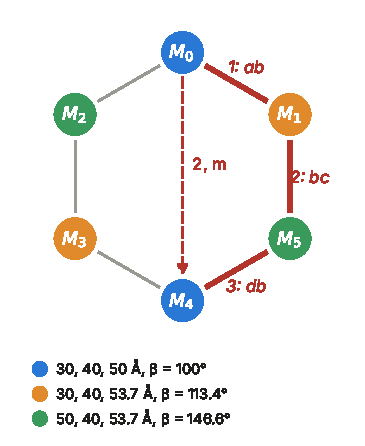
\includegraphics[width=0.45\textwidth]{figures/fig1_ring.pdf}
\caption{The closure of the $100^\circ$ cell: six objects on a ring, joined by flips at the two zero conorms and coloured by cell shape. The twofold and the mirror carry $M_0$ to $M_4$ along the flips $ab$, $bc$, $db$ followed by a swap, so they are arrows between objects rather than relabellings of $M_0$.}
\label{fig:ring}
\end{figure}

The point group is $2/m$, and each of its four operations is an arrow out of $M_0$ (last column of Table~\ref{tab:mono}).\chk{z46} The identity and the inversion are swaps of $M_0$. The twofold sends $(a,b,c)\mapsto(-a,b,-c)$ and so carries $(-a-b-c,a,b,c)$ to $(a-b+c,-a,b,-c)$: not a relabelling of $M_0$ but the object $M_4$, three flips away. As a word it is the flips $ab$, $bc$, $db$ --- the path $M_0\to M_1\to M_5\to M_4$ --- followed by the swap $-(a,c,b,d)$; the mirror is the same flips with the swap $(a,c,b,d)$.\chk{z46} Half of the point group is therefore invisible in the reduced cell: it consists of arrows between objects. ``Visible'' means only that an operation relabels the reduced superbase; a search over lattice directions, as Le Page's, finds the twofold either way.

\subsection{The universal operator set}
\label{sec:universal}
The arrows can be characterised with no lattice at all. An integer matrix $\Wop$ acts on the six conorms by a fixed integer $6\times6$ matrix, and $\Wop$ is an arrow of the closure of every lattice with zero pattern $Z$ exactly when that matrix maps the face $\{p\ge0,\ p_Z=0\}$ into the cone of non-negative conorms, a sign condition enumerated exactly (Appendix~D). The union over the 38 faces is a set $\mathcal U$ of $6096=48\times127$ integer matrices with entries in $\{-3,\dots,3\}$, closed under inversion, containing every arrow between two reduced cells of any lattice.\chk{z52} Up to swaps it has 127 elements; the superbases $\mathcal U F_0$ are every superbase that can be obtuse together with $F_0$ for some metric. This set carries the completeness statements of Section~\ref{sec:measured}.

%==============================================================================
\section{Measured cells: the widened groupoid}
\label{sec:measured}
%==============================================================================

A measured cell is never exactly on a zero conorm: a right angle is measured as $90.25^\circ$ and the conorm is a small number of either sign. The flips that joined the objects of Table~\ref{tab:mono} now lead to superbases with a slightly negative conorm, Selling reduction rejects them, and the exact closure of the measured metric has one object instead of six; the twofold and the mirror, which were arrows to $M_4$, now lead to a cell outside the set. The closure has to be widened.

\subsection{The strain norm}
\label{sec:strain}
The measure used is the relative change of the metric tensor,
\begin{equation}
\|\Delta\Gmet\|_{\Gmet}=\|\Gmet^{-1/2}\,\Delta\Gmet\,\Gmet^{-1/2}\|_F ,
\label{eq:strain}
\end{equation}
a strain: the affine-invariant norm on positive definite matrices (Pennec \emph{et al.}, 2006), to first order in $\Delta\Gmet$. It is unchanged by a change of basis, since $\Gmet\mapsto\Pop^{\mathsf T}\Gmet\Pop$ and $\Delta\Gmet\mapsto\Pop^{\mathsf T}\Delta\Gmet\Pop$ leave it as it is, so it is the same in every frame and every arrow of the closure is an isometry for it. A perturbation of norm $\epsilon$ changes the dot product of any two lattice vectors by at most $\epsilon|u||v|$ (Proposition~A4), so an angle by at most about $\epsilon$ radians and a squared edge by at most a fraction $\epsilon$, whatever the shape of the cell. A band on the conorms in \Ang$^2$, the measure of the first version of this work (Appendix~B), is the wrong measure for a cell whose edges differ in length: for a needle the error on the conorm between the two long vectors is hundreds of times that between the short ones, and in which frame a conorm is read changes its band.

The classical tolerances become one kind of number in this norm. Changing the angle between two vectors by $\delta$ is a strain of $\sqrt2\sin\delta$, and changing one edge by a fraction $f$ a strain of about $2f$; Le Page's $3^\circ$ (Le Page, 1982) and a $5\%$ edge tolerance are strains of $0.074$ and $0.10$. With a covariance for the metric tensor in place of a fixed norm, the same distances become $\chi^2$ statistics.

\subsection{The widened set}
\label{sec:widened}
The \emph{widened closure} of a metric $\Gmet$ at band $\epsilon$ is
\begin{equation}
\Se(\Gmet)=\bigl\{\,F\;:\;F\ \text{is obtuse for some metric within}\ \epsilon\ \text{of}\ \Gmet\ \text{in the norm~(\ref{eq:strain})}\,\bigr\}.
\label{eq:def}
\end{equation}
Its objects are the reduced cells of every lattice consistent with the measurement at band $\epsilon$; its arrows are the integer matrices between them, each with a \emph{price}, the strain $\|\Pop^{\mathsf T}\Gmet\Pop-\Gmet'\|_{\Gmet'}$ by which it fails to carry one metric onto the other. The arrows of price at most $\epsilon$ that carry the measured cell onto itself replace the point group. All arrows still compose, but the price of a product of two arrows is bounded only by the sum of their prices (the triangle inequality), so the arrows within the band at one object need not form a group; they form one when the band lies in a gap of the cell's sort spectrum (Section~\ref{sec:spectrum}). The depth of a superbase is measured at the measured metric and the price of an operator at its target; the two agree to first order in $\epsilon$ (Corollary~A8). The \emph{depth} of a superbase is its strain distance to the nearest metric that makes it obtuse, a non-negative least-squares problem in its six conorms; a superbase belongs to $\Se(\Gmet)$ when its depth is at most $\epsilon$, and its depth is the band at which it enters. Equation~(\ref{eq:def}) names no starting cell, order of operations or frame, so $\Se(\Gmet)$ is the same whoever computes it. Two properties make it computable and useful.

\emph{It is finite.} Every vector of a superbase in $\Se(\Gmet)$ lies in a ball of squared radius $\frac{1+\epsilon}{1-\epsilon}\mu_c$ about the origin, with $\mu_c$ the squared length of the shortest lattice vector in its parity class (Lemma~A6); the lattice vectors in these seven balls are finitely many, so $\Se(\Gmet)$ is enumerated exactly, with no window of coordinates to assume.

\emph{Widening one side suffices.} If a new cell, carried to a reference by an operator $\Pop$, differs from it by at most $\epsilon$, the new cell's reduced superbase, carried by $\Pop$, lies in the reference's widened closure (Corollary~A8). So the reference alone is widened and the new cell is reduced once.

\subsection{Computing the widened set}
\label{sec:snap}
For a measured cell and a band $\epsilon<1$:
\begin{enumerate}
\item Selling-reduce the measured cell to a superbase $F_0$.
\item Enumerate the lattice vectors in the seven balls of Lemma~A6 and form the superbases they make.
\item Keep the superbases of depth at most $\epsilon$. Record each one's depth and the operator $\Wop$ from $F_0$ to it.
\end{enumerate}
This is exact for every cell and every band. It is also more than is needed for most cells, and the layers of the universal set say how much. Call two superbases \emph{adjacent} when some metric makes both obtuse; the superbases adjacent to $F_0$ are the first layer $\Lay_1=\mathcal U F_0$, 127 superbases up to relabelling, and $\Lay_k=\mathcal U\Lay_{k-1}$, with 2755 in the second layer.\chk{z59} The \emph{adjacency radius} $\delta_k(\Gmet)$ is the strain distance from $\Gmet$ to the nearest metric for which a superbase outside $\Lay_k$ is obtuse, computed exactly from the balls of Lemma~A6 at $\epsilon=\frac14$. If $\epsilon<\min(\delta_k,\frac14)$, the widened set is the filtered $k$th layer (Theorem~A7): its members are the superbases of $\Lay_k$ of depth at most $\epsilon$. The \emph{tier} of a cell at band $\epsilon$ is the least $k$ for which the widened set lies in $\Lay_k$. In \emph{tier 1} the candidates are the 127 superbases of the first layer, filtered; this holds whenever $\epsilon$ is below $\delta_1$, which for cells of ordinary shape exceeds a quarter strain, about $10^\circ$ (Section~\ref{sec:complete}). In \emph{tier 2}, needles and plates whose $\delta_1$ is below the band but $\delta_2$ above it, it lies in the second layer; beyond $\delta_2$, in \emph{tier 3}, the balls of Lemma~A6 are enumerated directly. The tier records how far the set had to reach, not how far it can be trusted.

A constructive alternative builds the set from the lattices near the measurement: for each of the 127 frames of the first layer and each of the 38 faces of the cone, project the measured metric onto the face (the nearest metric in the norm~(\ref{eq:strain}) with those conorms zero and the others non-negative); for every projection within $4\epsilon$ (the proof needs $\epsilon$; the factor is a margin), enumerate the exact closure of the projected lattice; keep the members of depth at most $\epsilon$; take the union. Below $\delta_1$ this returns $\Se(\Gmet)$ (Theorem~A7). A single projection, onto the most special face within $4\epsilon$, is not enough (Section~\ref{sec:complete}).

\emph{Ties take no band.} Only zeros enter the construction. Every sort lies on one zero pattern, and every symmetry of every lattice on that pattern is one of its arrows (Lemma~A3), so a near-equality --- the $a\approx b$ of a pseudo-tetragonal cell --- never adds a superbase: the operator that would be its symmetry is already enumerated, and whether it is accepted is decided by its price.

\subsection{Distance to each sort}
\label{sec:spectrum}
The same norm measures how far a measured cell is from each of the 24 sorts: project its conorms, in each of the 6096 frames of $\mathcal U$, onto the sort's subspace of Proposition~A5 (its zeros and equalities, the other conorms non-negative), and take the smallest distance. Projection onto Bravais-lattice subspaces is the approach of Andrews \& Bernstein (2014) in $G^6$ and of Oishi-Tomiyasu (2012) in Selling coordinates; here the frames are the complete finite set of the closure and the norm is the same in every frame. We call the 24 distances the \emph{sort spectrum} of the cell. A cell idealised onto one sort can be projected again onto the next; the step between two sorts joined by a specialisation (Table~\ref{tab:special}) is the distance from the idealised upper sort to the lower one.

\subsection{Reindexing}
\label{sec:reindex-method}
A reference $R$ is stored as its widened closure, the operators $\Wop_k$ from its reduced cell to the members. A new cell $N$ is reduced once, to a basis $B_N$ in its own coordinates; $B_R$ is the reduction matrix of the reference. For each stored $\Wop_k$ and each of the 48 swaps $\mathbf Q$ the candidate operator from the reference's input basis to the new cell's is
\begin{equation}
\Pop=B_R\Wop_k\mathbf Q\,B_N^{-1},
\label{eq:candidate}
\end{equation}
so that $(a_N\,b_N\,c_N)=(a_R\,b_R\,c_R)\Pop$, $\Gmet_N\approx\Pop^{\mathsf T}\Gmet_R\Pop$ and Miller indices transform as $h_N=\Pop^{\mathsf T}h_R$. Each candidate is priced by $\|\Pop^{\mathsf T}\Gmet_R\Pop-\Gmet_N\|_{\Gmet_N}$ after the common scale that best fits the two metrics in the Frobenius norm, since a detector distance or wavelength error scales every conorm; candidates of price at most $\epsilon$ are returned. Centred cells are first taken to primitive cells and the centring matrices composed with the operator found; the result is carried to the conventional setting of the target space group outside the closure. Candidates of determinant $-1$ are discarded for a chiral crystal.

The candidates are one coset $\Pop_0H_\epsilon$, with $H_\epsilon$ the arrows of price at most $\epsilon$ that carry the reference onto itself, a group whenever the band lies in a gap of the cell's sort spectrum. Two candidates that differ on the left by an element of the reference's Laue group $\Laue$ index the crystal the same way, so the distinct indexings are the $[H_\epsilon:\Laue]$ classes of $\Laue$ in the coset. Membership of the true operator is what is guaranteed; the price orders the candidates but does not single out the true one within its coset, which is a matter for the intensities, as in a twinning test. The procedure is implemented as \texttt{agentsg.cell.strain\_closure}, with \texttt{widened\_closure}, \texttt{reindex}, \texttt{indexing\_classes} and \texttt{sort\_spectrum}.

\subsection{Verification}
\label{sec:verification}
Exact closures and the closures of the 24 sorts were checked against brute force over every basis with coordinates in $[-2,2]$ relative to $F_0$, a window that contains every member of every exact closure (Lemma~A1).\chk{z52} Widened sets were checked against the ball enumeration of Lemma~A6, which needs no window, and against brute force over $[-3,3]$ for needles and plates.\chk{z58,z59} Test lattices were specified by their conorms. The measured worked cell is $30.02$, $39.97$, $50.03$\,\Ang, $90.25^\circ$, $92.05^\circ$, $89.80^\circ$: the $100^\circ$ cell of Section~\ref{sec:example} with $\beta$ moved to $92^\circ$, so that it sits on two zero conorms and near a third, perturbed by a metric error of $14.4$\,\Ang$^2$ in Frobenius norm. A benchmark of 780 measured cells with exact references and true operators, built where the closure predicts trouble, is described in Appendix~C. The checks are the test files of Appendix~E.

%==============================================================================
\section{Results}
\label{sec:results}
%==============================================================================

\subsection{The closures of the 24 sorts}
\label{sec:groupoid}
For each zero pattern $Z$ the arrows are the operators of the universal set that map the face of $Z$ into the cone; on the face every arrow permutes the six conorm slots, so each fixes a subspace of conorm vectors, and the sorts are the closed sets of equalities obtained by intersecting those subspaces (Proposition~A5). For a sort, the point group is the set of arrows that fix the sort's subspace pointwise, the visible symmetries are those that are swaps of the reduced cell, and two objects have the same shape when their conorms agree up to a slot permutation. Every entry of Table~\ref{tab:sorts} is the result of this linear algebra on integer matrices.\chk{z54} Out of each object there are exactly as many symmetries as the point group has elements, and in every sort that number is the order of the holohedry: 48, 24, 16, 12, 8, 4 or 2. The twofolds, with the inversion, generate the group in every sort, so finding the twofolds suffices.\chk{z46}

\begin{table}
\caption{The Selling closure of each Delone sort, computed from the operators alone. Patterns are Selling parameters in the $S^6$ order $b\cdot c, a\cdot c, a\cdot b, a\cdot d, b\cdot d, c\cdot d$; equal letters denote equal values and $0$ a zero. Objects are counted up to swaps. ``Visible'' is the number of symmetries that relabel the reduced superbase; the rest carry it to another object. ``Shapes'' is the number of distinct cell shapes among the objects, equal in every case to the number of orbits of objects under the symmetries. ``Visible'' depends on which object one reduces to; values are for the pattern as written.\chk{z54}}
\label{tab:sorts}
\begin{footnotesize}
\begin{tabular}{llcccccc}
\toprule
sort & Bravais & pattern & zeros & objects & $|$group$|$ & visible & shapes \\
\midrule
C1 & cI & rrrrrr & 0 & 1 & 48 & 48 & 1 \\
C3 & cF & rr0rr0 & 2 & 3 & 48 & 16 & 1 \\
C5 & cP & 000rrr & 3 & 16 & 48 & 12 & 2 \\
H4 & hP & 00rrrs & 2 & 6 & 24 & 4 & 1 \\
T1 & tI & rrsrrs & 0 & 1 & 16 & 16 & 1 \\
T2 & tI & rr0rrs & 1 & 2 & 16 & 8 & 1 \\
T5 & tP & 000rrs & 3 & 16 & 16 & 4 & 3 \\
R1 & hR & rrrsss & 0 & 1 & 12 & 12 & 1 \\
R3 & hR & rr0sr0 & 2 & 3 & 12 & 4 & 1 \\
O1A & oF & rrsrrt & 0 & 1 & 8 & 8 & 1 \\
O1B & oI & rstrst & 0 & 1 & 8 & 8 & 1 \\
O2 & oI & rs0srt & 1 & 2 & 8 & 4 & 1 \\
O3 & oI & rs0rs0 & 2 & 3 & 8 & 8 & 2 \\
O4 & oS & 00rsst & 2 & 6 & 8 & 4 & 2 \\
O5 & oP & 000rst & 3 & 16 & 8 & 2 & 4 \\
M1A & mC & rrsttu & 0 & 1 & 4 & 4 & 1 \\
M1B & mC & rstrsu & 0 & 1 & 4 & 4 & 1 \\
M2A & mC & rs0stu & 1 & 2 & 4 & 2 & 1 \\
M2B & mC & rs0rst & 1 & 2 & 4 & 4 & 2 \\
M3 & mC & rs0ts0 & 2 & 3 & 4 & 4 & 2 \\
M4 & mP & 00rstu & 2 & 6 & 4 & 2 & 3 \\
A1 & aP & rstuvw & 0 & 1 & 2 & 2 & 1 \\
A2 & aP & rs0tuv & 1 & 2 & 2 & 2 & 2 \\
A3 & aP & rs0tu0 & 2 & 3 & 2 & 2 & 3 \\
\bottomrule
\end{tabular}
\end{footnotesize}
\end{table}

\emph{Zero pattern and sort fix different parts.} Which objects exist and which arrows join them is fixed by the zero pattern; which arrows are symmetries is fixed by the sort, and the abstract group by the Bravais type. Primitive monoclinic, C-centred orthorhombic and primitive hexagonal lattices all have two zeros sharing a vector and six objects, and differ only in how many arrows are symmetries (4, 8, 24). Within one sort the shape of the cell plays no part: the objects, arrows and symmetries are the same, and the lattice supplies only the numbers attached to them.

\emph{Symmetry visible in one cell.} In the sorts with zero conorms the symmetries that relabel the reduced cell are a minority: 2 of 8 for primitive orthorhombic, 4 of 16 for primitive tetragonal, 12 of 48 for primitive cubic, 4 of 24 for hexagonal, 4 of 12 for rhombohedral R3.\chk{z46} None of the three twofolds of a primitive orthorhombic lattice relabels its reduced cell, nor the one twofold of primitive monoclinic; of the five, nine and seven twofolds of primitive tetragonal, cubic and hexagonal lattices, one, three and one do.\chk{z46}

\emph{Cell shapes.} Two objects are related by a symmetry exactly when they have the same shape, so the number of shapes equals the number of symmetry orbits (last column of Table~\ref{tab:sorts}), and no symmetry relates cells of different shape.\chk{z54} Two measurements of the monoclinic lattice that reduce to $M_0$ and to $M_1$ report different cell parameters and are related by no symmetry, only by the flip at $ab$. Ten of the 24 sorts have more than one shape. Primitive orthorhombic has four: the orthogonal cell and three monoclinic-looking cells with two right angles, one for each axis traded for a face diagonal; reduction of a measured orthorhombic cell stops at whichever of the sixteen objects its errors favour, and the orthogonal cell is up to three flips away, reached by no twofold of the lattice. The three shapes of a primitive monoclinic lattice are the three cell choices of \emph{International Tables} (Hahn, 2006, Section~2.2.16); the catalogue is Table~\ref{tab:shapes} of Appendix~C.

\emph{Specialisations.} The same algebra gives the conditions under which a lattice of one sort becomes a lattice of another (Table~\ref{tab:special}, Appendix~C). Every condition of codimension one is a conorm vanishing or two conorms becoming equal; they join 36 pairs of sorts.\chk{z50} The classical values $c/a=\sqrt2$ (tI to cF), $b=\sqrt3\,a$ (oS to hP) and $a=c$ in a monoclinic cell are among them, and the monoclinic conditions come in threes, one per cell choice. The two kinds behave differently under error. A near-equality, such as $c/a\approx\sqrt2$, changes no zero pattern: the object set is already complete and the pseudo-symmetry appears as a priced arrow. A near-zero, such as a C-centred monoclinic cell one zero from primitive tetragonal, adds objects, and those are what the widened closure recovers.

\subsection{Distances to the sorts}
\label{sec:spectrum-results}
The sort spectrum orders the possible symmetry assignments of a measured cell in one unit. An oP cell $40.0\times40.3\times80$\,\Ang\ is $1.06\%$ from tP, the strain of its $0.75\%$ edge mismatch; a C-centred monoclinic cell $50\times86.8\times40$\,\Ang, $\beta=90.4^\circ$, is $1.04\%$ from hP; an F cell $100\times100.2\times99.9$\,\Ang\ is $0.43\%$ from cF.\chk{z58} Along every specialisation of Table~\ref{tab:special} the distance never decreases,\chk{z58} and in the two cells of Fig.~\ref{fig:sortgraph} the steps along the cheapest route add approximately in quadrature: the distance to a lower sort is close to $\sqrt{d^2+s^2}$, with $d$ the distance to the upper sort and $s$ the step.

Figure~\ref{fig:sortgraph} draws the spectrum on the graph of specialisations for two cells. For the worked cell the cheap route is A1 to A2 at $0.28\%$, then mP (M4) at $0.78\%$ and oP at $5.1\%$; every other sort is more than $30\%$ away.\chk{z60} For a tetragonal lysozyme cell indexed in $P1$ the twelve sorts from aP to tP all lie within $0.22\%$, and the next sort is $43\%$ away.\chk{z60} In both cells the sorts fall into a cluster and a gap, and the Bravais type is the last sort before the widest gap: mP for the worked cell, tP for lysozyme. The many C-centred sorts near lysozyme are no separate pseudo-symmetry: a square net has an equally good C-centred cell on its diagonals, so every tP lattice is also nearly oS and mC. Dashed edges keep the Bravais type and change only the reduced cell (A1 to A2 to A3, or between the mC sorts); they add objects to the closure but no symmetry.

\begin{figure}
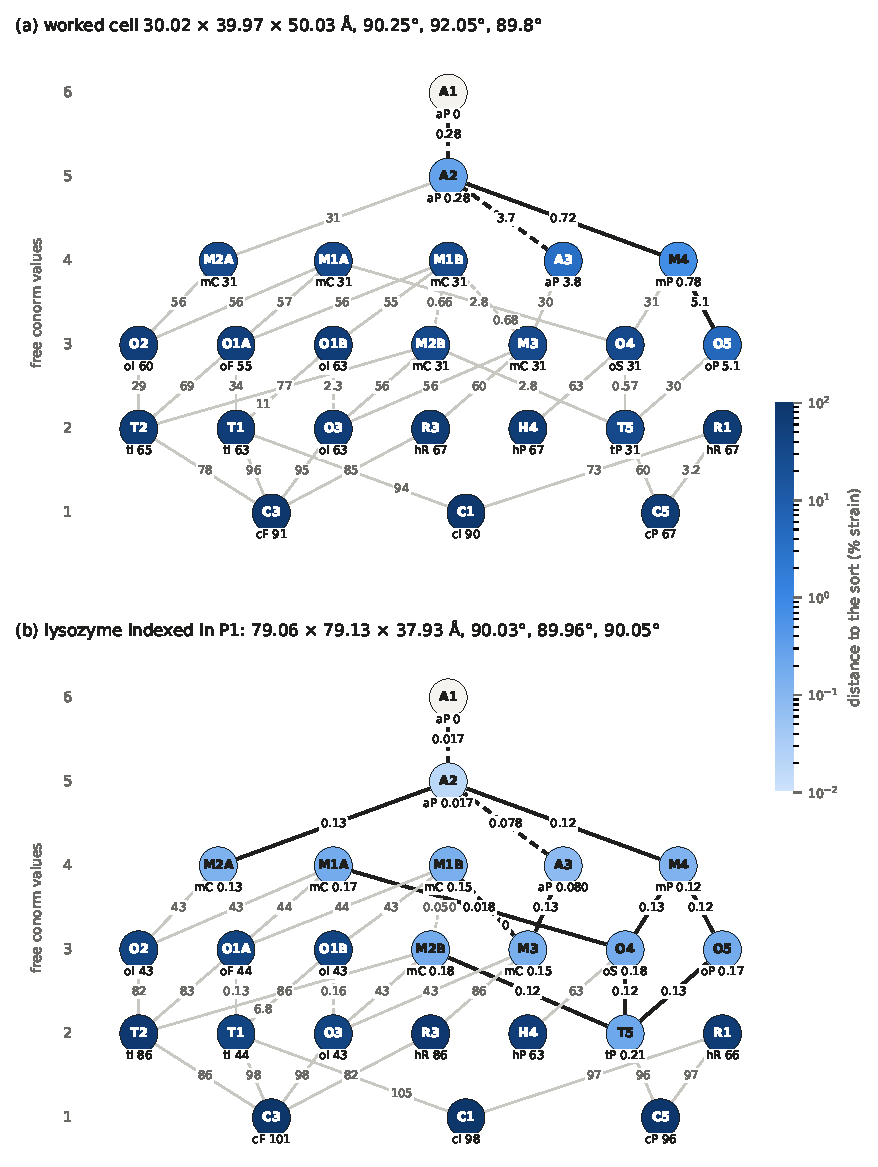
\includegraphics[height=0.72\textheight]{figures/fig3_sort_graph.pdf}
\caption{The 24 Delone sorts as a graph, for (\emph{a}) the measured worked cell and (\emph{b}) a tetragonal lysozyme cell indexed in $P1$ (a cell of $79.1\times79.1\times37.9$\,\Ang\ with an added error). Rows are the number of free conorm values. Nodes give the Bravais type and the strain distance (\%) from the measured cell to the sort; colour is the same distance on a log scale. Edges are the specialisations of Table~\ref{tab:special}, labelled with the step from the cell idealised onto the upper sort to the lower one. Dark edges are routes on which the steps add in quadrature to the lower sort's distance within $3\%$, drawn where that distance is below $10\%$. Dashed edges keep the Bravais type. The node distances are checked in [z60].}
\label{fig:sortgraph}
\end{figure}

The seven measured cells that Oishi-Tomiyasu (2024) distributes with her program give an independent check (Table~\ref{tab:conograph}). In every case Le Page's band, $0.074$, separates the program's Bravais type from the next type in the spectrum, and in six of the seven the program's type is the last before the widest gap; for the rhombohedral alumina cell the widest gap lies below hR, between mC at $0.43\%$ and hR at $3.58\%$, with the next type at $14.9\%$.\chk{z60} The program's distance is a norm in \Ang$^2$ on the metric tensor (Oishi-Tomiyasu, 2012) and the strain is relative, so the two agree in order, not in value.

\begin{table}
\caption{The seven sample cells of BLDConograph (Oishi-Tomiyasu, 2024): the program's Bravais type and minimal distance (\Ang$^2$); the strain distance (\%) from the cell to that type, and to the next type in the sort spectrum.\chk{z51,z60}}
\label{tab:conograph}
\begin{footnotesize}
\begin{tabular}{llrrlr}
\toprule
sample & type & program & strain & next type & strain \\
\midrule
HERMES\_Sr327\_250K & tI & 0.57 & 0.84 & mP & 25.6 \\
1339prbasrcuo\_bs1 & tP & 0.056 & 0.22 & oF & 31.5 \\
sample3 & cI & 2.07 & 0.58 & cF & 57.6 \\
CeO2\_matsushita & cF & 0.084 & 0.30 & cI & 47.0 \\
M402-pf-119673 & hP & 20.5 & 2.94 & oI & 33.8 \\
Acrinol-B-D8CuKa1 & mC & 0.72 & 0.31 & oF & 20.6 \\
Alumina676 & hR & 1.93 & 3.58 & oI & 14.9 \\
\bottomrule
\end{tabular}
\end{footnotesize}
\end{table}

\subsection{Completeness on measured cells}
\label{sec:complete}
\label{sec:nearcong}
\emph{A worked filter.} The reduced superbase of the worked cell has conorms $49.5$, $1588.9$, $2444.7$, $4.2$, $847.5$ and $4.5$\,\Ang$^2$ in the slots $da,db,dc,ab,ac,bc$. Its widened closure grows with the band: one member at $\epsilon=0.001$, two at $0.003$, three at $0.006$, the six of the ring from $0.01$, and sixteen at Le Page's $0.074$.\chk{z60} Table~\ref{tab:filter} lists the sixteen, each as a word in the flips of Table~\ref{tab:flips}, with its conorms under the measured metric and its depth (Fig.~\ref{fig:depths}). The six members of the ring enter below $0.8\%$; the other ten members of the closure of the nearby orthorhombic lattice enter between $3.8$ and $5.1\%$. Depths are not ordered as the most negative conorms are --- $da$, with $-49.5$\,\Ang$^2$, enters before $da.ab.bc$, with $-45.0$ --- because the strain weighs each conorm by the lengths of the vectors it joins.

\begin{table}
\caption{The widened closure of the measured worked cell. Each row is a member, named by a word in the flips of Table~\ref{tab:flips} from the reduced cell $e$; the six numbers are its conorms under the measured metric, slots $da,db,dc,ab,ac,bc$, in \Ang$^2$; ``depth'' is the strain at which it enters, in \%. At Le Page's band, $7.4\%$, all sixteen are members.\chk{z45,z60}}
\label{tab:filter}
\begin{footnotesize}
\begin{tabular}{lrrrrrrr}
\toprule
word & $da$ & $db$ & $dc$ & $ab$ & $ac$ & $bc$ & depth \\
\midrule
$e$ & 49.5 & 1588.9 & 2444.7 & 4.2 & 847.5 & 4.5 & 0 \\
$bc$ & 45.0 & 8.7 & 2449.3 & 1593.4 & 852.0 & $-4.5$ & 0.28 \\
$ab$ & 851.7 & 1593.1 & 2440.6 & $-4.2$ & 53.7 & 8.7 & 0.49 \\
$bc.db$ & 2458.0 & $-8.7$ & 53.7 & 1602.1 & 843.3 & 4.2 & 0.62 \\
$ab.bc$ & 842.9 & 4.5 & 2449.3 & 1601.8 & 62.5 & $-8.7$ & 0.78 \\
$ab.bc.db$ & 2453.8 & $-4.5$ & 847.5 & 1606.3 & 57.9 & $-4.2$ & 0.78 \\
\midrule
$da$ & $-49.5$ & 2494.3 & 1638.4 & 53.7 & 897.0 & $-45.0$ & 3.76 \\
$ab.bc.ac$ & 1664.2 & $-57.9$ & 2511.7 & 905.4 & $-62.5$ & 53.7 & 4.56 \\
$da.ab$ & 950.7 & 2548.0 & 1584.7 & $-53.7$ & 4.2 & 8.7 & 5.06 \\
$da.ab.ac$ & $-49.5$ & 2543.8 & 1588.9 & 954.9 & $-4.2$ & 12.9 & 5.08 \\
$ab.ac$ & 49.5 & 1539.3 & 2494.3 & 905.4 & $-53.7$ & 62.5 & 5.08 \\
$da.ab.bc$ & 942.0 & $-45.0$ & 1593.4 & 2556.7 & 12.9 & $-8.7$ & 5.09 \\
$bc.db.dc$ & 45.0 & 2511.7 & $-53.7$ & 1548.4 & 897.0 & 57.9 & 5.09 \\
$ab.ac.bc.ac$ & 1610.5 & 959.1 & 2565.5 & $-4.2$ & $-8.7$ & $-53.7$ & 5.11 \\
$da.ab.bc.ac$ & 2569.6 & $-57.9$ & 1606.3 & 954.9 & $-12.9$ & 4.2 & 5.11 \\
$ab.ac.bc$ & $-12.9$ & 967.8 & 2556.7 & 1601.8 & 8.7 & $-62.5$ & 5.11 \\
\bottomrule
\end{tabular}
\end{footnotesize}
\end{table}

\begin{figure}
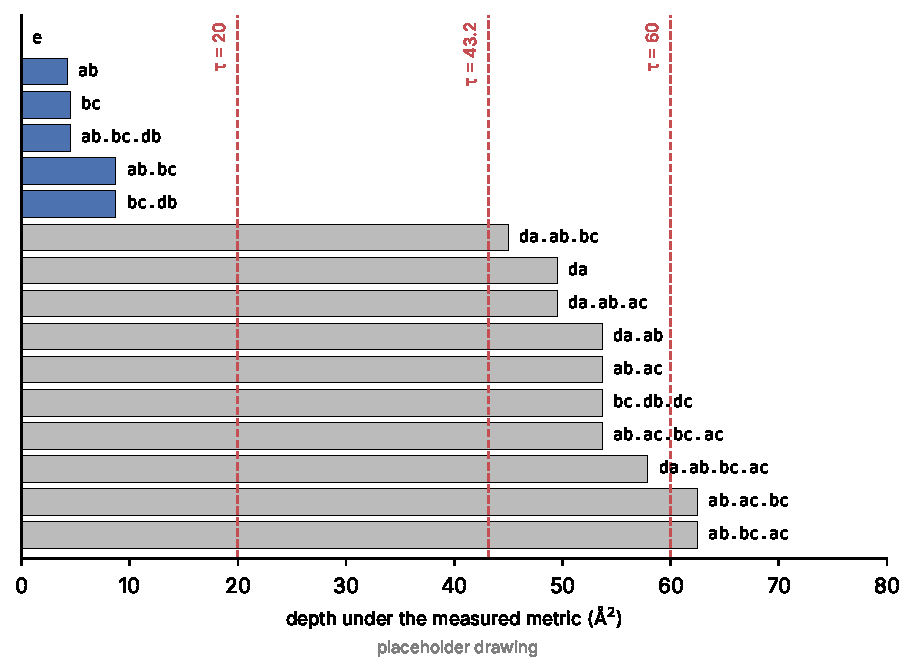
\includegraphics[width=0.6\textwidth]{figures/fig2_depths.pdf}
\caption{The sixteen members of the widened closure of the measured worked cell (Table~\ref{tab:filter}) by depth: the six of the ring enter below $0.8\%$ strain, the other ten members of the nearby orthorhombic lattice's closure between $3.8$ and $5.1\%$; the band selects among them.\chk{z60}}
\label{fig:depths}
\end{figure}

\emph{The set has to be computed, not sampled.} Reduction with a widened boundary does not stop at a well-defined cell. With a band on the conorms (Appendix~B), reduction of the worked cell and of a noisy orthorhombic cell from random starting bases stopped at several different members of the widened set, and on a noisy cubic cell the restarts did not find all of them.\chk{z45} Walks from the measured reduced cell, flipping wherever a conorm is within a band of zero, miss members too; with the conorm band, on 80 cells with zero conorms at awkward positions, four versions of the walk returned a wrong set on 2 to 13 cells (Table~\ref{tab:walks}). The cause is a member reachable only through a non-member, for instance when two small conorms lie at $1.2$ and $0.5$ times the band, where the flip across the first leaves the band and only a second flip, across the other, returns into it.\chk{z44,z45} Such \emph{difference-wall members} carry no symmetry; they are ordinary alternative reduced cells to which a second measurement can reduce, and a reference set built by walking never contains them.\chk{z46}

\begin{table}
\caption{Four walks on the measured metric, and the construction of Appendix~B, against brute force on 80 cells with zero conorms at awkward positions (orthorhombic, cubic, plate, monoclinic and hexagonal zero patterns), with a band $\tau$ on the conorms at $0.1$ and $0.5$ of $\lambda_1/32$.\chk{z45}}
\label{tab:walks}
\begin{tabular}{lc}
\toprule
procedure & cells with a wrong set \\
\midrule
flip wherever $|p|\le\tau$, keep only cells within the band & 13 \\
flip wherever $|p|\le\tau$, filter at the end & 13 \\
flip wherever $|p|\le2\tau$, keep only cells within the band & 13 \\
flip wherever $|p|\le2\tau$, filter at the end & 2 \\
idealise at $4\tau$, enumerate the exact closure, filter & 0 \\
\bottomrule
\end{tabular}
\end{table}

\emph{Needles and plates.} A band on the conorms has to cover the conorms between the long vectors of a needle, and the proved conorm-band construction of Appendix~B then fails at a few thousandths of a degree. Bands per slot, $\sigma|u_i||u_j|$, applied in the frame of the reduced cell, are not exact either: the needle $5.58\times5.21\times131.97$\,\Ang, $\gamma=91.12^\circ$, at $\sigma=\sin0.064^\circ$ gives 6 superbases where the per-slot widened set has 12, because on the slot $(a+c,b)$ of the missing members the same dot product carries a much larger band.\chk{z57} The strain norm has no frame-dependent band. The projection construction of Section~\ref{sec:snap} returned the exact set for this needle at $\epsilon=0.0005$, $0.002$, $0.005$, $0.01$, $\sin1^\circ$ and $\sin3^\circ=0.052$; for a $100\times100.1\times5$\,\Ang\ plate and a $150\times120\times4.8$\,\Ang\ plate, $\beta=90.4^\circ$, at $\epsilon=0.052$, where their widened sets have 20 and 28 members, more than any single closure; and for 60 random needles, plates, isotropic and monoclinic cells at four bands each, $\sin0.1^\circ$ to $\sin3^\circ$, in all 240 cases.\chk{z58,z60} A single projection onto the most special face is not enough: on the needle at $\epsilon=0.002$ and $0.005$ it returns 6 of the 8 members, missing those built on $a+c$, which belong to a lattice in which $(a+c)\cdot b$, not $a\cdot b$, is zero.\chk{z60}

\emph{How far the proof reaches.} Table~\ref{tab:radii} gives the adjacency radii. For cells of ordinary shape no superbase outside the first layer comes within a quarter strain, so tier 1 holds at every band in use. For needles and plates $\delta_1$ falls with the ratio of the shortest to the longest edge, between one and $\sqrt2$ times that ratio in the cells of Table~\ref{tab:radii}, and the second layer roughly doubles it. The two plates at $\epsilon=0.052$ lie between $\delta_1$ and $\delta_2$: the first layer misses members there, and the second contains them all, as Theorem~A7 requires.\chk{z59} Their $\delta_2$ also exceeds Le Page's $0.074$, so at that band too the filtered second layer is their widened set. The number of layers a band needs is therefore the measure of a cell's difficulty, in place of a single angular limit.

\begin{table}
\caption{Adjacency radii in the strain norm~(\ref{eq:strain}): $\delta_1$, the smallest strain at which a superbase outside the first layer becomes obtuse, and $\delta_2$ for the second layer. The search is capped at $0.25$. Le Page's $3^\circ$ is a strain of $0.074$.\chk{z59}}
\label{tab:radii}
\begin{tabular}{lcc}
\toprule
cell & $\delta_1$ & $\delta_2$ \\
\midrule
$30\times40\times50$\,\Ang, $\beta=92^\circ$ (the worked cell) & $>0.25$ & $>0.25$ \\
needle $10\times10\times30$\,\Ang\ & $>0.25$ & $>0.25$ \\
needle $10\times10\times100$\,\Ang\ & $0.139$ & $>0.25$ \\
needle $5.58\times5.21\times132$\,\Ang, $\gamma=91.12^\circ$ & $0.056$ & $0.111$ \\
plate $100\times100.1\times5$\,\Ang\ & $0.050$ & $0.141$ \\
plate $150\times120\times4.8$\,\Ang, $\beta=90.4^\circ$ & $0.043$ & $0.100$ \\
\bottomrule
\end{tabular}
\end{table}

\subsection{Reindexing}
\label{sec:reindex}
\emph{Indexing classes.} Figure~\ref{fig:classes} shows the classes for six references, each against the same crystal measured again with a $0.1\%$ error in the length scale. Tetragonal lysozyme in $P4_32_12$ has one class: no ambiguity. $P3$ has four, joined by the twofolds along $[001]$, $[110]$ and $[1\bar10]$, the classical indexing ambiguities of that group; $P3_121$ and $P2_13$ have two, joined by one merohedral twofold. A pseudo-tetragonal $P2_12_12_1$ cell, $40.0\times40.3\times80$\,\Ang, and the worked cell in $P1$ each have a second class at a price, $2.11\%$ and $1.55\%$: the twofold that would make the cell tetragonal or monoclinic. That price is twice the cell's distance to the sort the twofold fixes, $1.06\%$ and $0.78\%$,\chk{z60} as for a reflection, whose image of a point lies twice as far from it as the mirror does; a pseudo-symmetry enters the candidates when its sort lies within half the band. A pseudo-merohedral ambiguity is therefore a priced alternative rather than a free one.

\begin{figure}
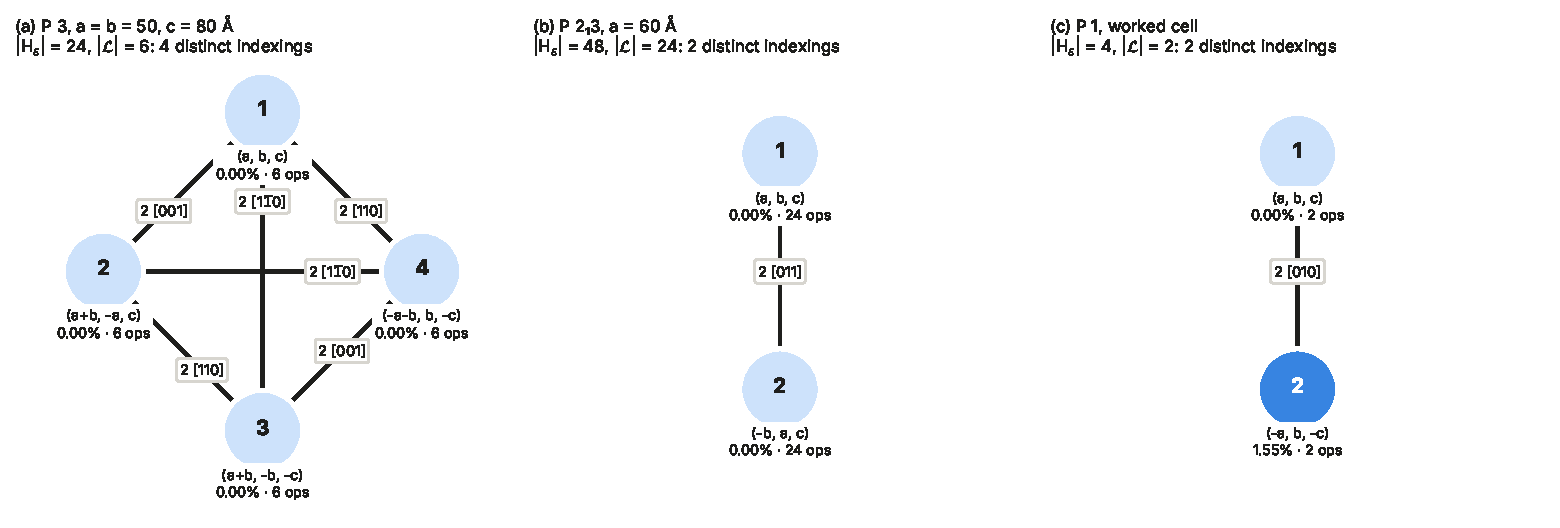
\includegraphics[width=\textwidth]{figures/fig4_indexing_classes.pdf}
\caption{Distinct indexings as the classes of the Laue group $\Laue$ in the band's coset, at Le Page's band, for six references measured again with a $0.2\%$ scale error. Each node is one class; it shows the class's operator nearest the identity (new basis in terms of the reference's $a$, $b$, $c$), its strain price and the number of operators in it. Each edge is the lattice symmetry or pseudo-symmetry carrying one class to the other, as rotation order and axis $[uvw]$ in the reference basis. Node colour is the price, from $0$ (light) to $3\%$.}
\label{fig:classes}
\end{figure}

\emph{The benchmark.} On the 780 constructed cases of Appendix~C, with the reference widened at Le Page's band and the new cell reduced once, the true operator was among the candidates in all 780; at a band of three times each case's own error strain it was found in all 779 cases in which that band is below a quarter (\texttt{manuscript/benchmark/results\_strain.txt}). The anisotropic family of 16 needles and plates fell in tier 2 in 12 cases and tier 1 in 4; no case was refused, where the conorm-band construction declined 8 of them. The median number of candidates was 8. For comparison, a symmetry-only reindexing, which pairs the new reduced cell with the reference's reduced cell in its 48 labellings, proposes the true operator in 54\% of the cases, and the exact closure without widening in 96\%. The same cases show where the Niggli cell is unstable: the measured cell's Niggli cell is a different cell from the reference's in 45 of 780, nearly all at the body-centred orthorhombic sort O3 and its neighbours, where two shapes of one closure are chosen by the sign of a near-zero quantity (\texttt{evaluate.py --niggli}). The benchmark is built where the closure predicts trouble, so these are rates on constructed cases, not in the wild.

\emph{Completeness of the stored set matters.} A new cell constructed so that its only reduced superbase is a difference-wall member of an orthorhombic corner was matched, with the conorm band of Appendix~B, against two stored sets of the reference. The complete set offers three candidates and their negatives; a set built by idealising only at the band has lost the third, which is $\pm\mathbf I$, the true operator.\chk{z46} The cheapest candidate is found either way, through a pseudo-symmetry, but it is not the true operator: price orders the coset, it does not identify its true member.

%==============================================================================
\section{Discussion}
\label{sec:discussion}
%==============================================================================

\emph{Where reindexing has been hard.} The usual pipeline reduces a cell, idealises it to the highest Bravais lattice within a tolerance (Le Page, 1982; Sauter \emph{et al.}, 2004) and standardises to a conventional cell; two data sets so treated agree unless they idealise to different lattices or fall on opposite sides of a tie in the standardisation. What the symmetry step cannot propose is the flip at $ab$, because it is a symmetry of nothing. That flip separates $c$ from $a+c$, the orthogonal cell from its monoclinic-looking shapes, and the two reduced cells of the sort O3 that two measurements return. The closure adds exactly those operators, with the pseudo-symmetries, each priced, and its gain over the pipeline is the completeness statement, not a higher hit rate on ordinary cells. Table~\ref{tab:traps} collects the traps, where each is found and what resolves it.

\begin{table}
\caption{The reindexing traps as the closure finds and resolves them.}
\label{tab:traps}
\begin{footnotesize}
\begin{tabular}{>{\raggedright\arraybackslash}p{2.8cm}>{\raggedright\arraybackslash}p{4.0cm}>{\raggedright\arraybackslash}p{2.3cm}>{\raggedright\arraybackslash}p{3.5cm}}
\toprule
trap & mechanism & found & resolved by \\
\midrule
monoclinic $c$ versus $a+c$ & flip at the zero conorm $ab$; two shapes, no symmetry between them & Sec.~\ref{sec:example}, Table~\ref{tab:mono} & both shapes are objects of the closure \\
oP, tP, cP reported as a monoclinic cell & twelve of sixteen objects lie on face diagonals & Sec.~\ref{sec:groupoid}, Table~\ref{tab:filter} & the widened closure; the orthogonal cell and its twofolds enter at a depth \\
pseudo-merohedry & a near-equality leaves the object set complete; a near-zero adds objects & Sec.~\ref{sec:groupoid}, Fig.~\ref{fig:classes} & prices; indexing classes \\
Niggli-cell instability (O3 and neighbours) & two shapes of one closure chosen by the sign of a near-zero & Sec.~\ref{sec:reindex} & both shapes stored \\
difference-wall member & reachable only through a non-member & Sec.~\ref{sec:complete}, Table~\ref{tab:walks} & enumerate the set, do not walk \\
needles and plates & a conorm's error depends on the slot and the frame & Sec.~\ref{sec:complete}, Table~\ref{tab:radii} & strain norm; second layer \\
choice within the coset & the metric cannot separate an operator from its product with a (pseudo-)symmetry & Sec.~\ref{sec:reindex} & not by the metric: intensities \\
\bottomrule
\end{tabular}
\end{footnotesize}
\end{table}

\emph{The Niggli cell.} The instability of the Niggli cell (Andrews \emph{et al.}, 1980; Andrews \& Bernstein, 1988, 2014) is the same phenomenon only in part. Andrews \& Bernstein locate it at every boundary of the Niggli cone: the sign boundary between type I and type II, the ties $a=b$ and $b=c$, and the special conditions. Only the boundaries at a zero scalar product are zero conorms; a tie is not, and the type I/II change gives a cell of the same lengths and supplementary angles, which in the closure is one shape and a swap. The Selling-reduced cell shares the instability at zero conorms, as Andrews \emph{et al.} (2019\emph{b}) note; what the closure adds is not stability of any one cell but completeness of the set of alternatives, so that two data sets reduced either way are related by a stored operator. Tolerant Niggli reduction (K\v{r}iv\'y \& Gruber, 1976; Grosse-Kunstleve \emph{et al.}, 2004) returns one of these cells, not the set.

\emph{Distances and symmetry assignment.} The sort spectrum is the measurement's distance to every symmetry it could be assigned, in one unit and in every frame. It agrees in order with the Bravais-type distances of Oishi-Tomiyasu (2012, 2024) and the quality indices of Kabsch (1993), and the gap in the spectrum gives a band that does not have to be chosen in advance: a band inside a gap gives the same symmetry assignment at any value in it. SELLA (Andrews \emph{et al.}, 2023) carries the boundary images of a cell to measure its distance to each sort in $S^6$; the frames here are the finite universal set, and the price of each operator is reported with it. The twofolds are the operators that matter: their prices, twice the distance to the sort they fix, rank the pseudo-symmetries as the tolerance-ranked subgroups of Sauter \emph{et al.} (2004) and the twinning operators of Lebedev \emph{et al.} (2006) do, and the indexing classes are the twin laws of the reference.

\emph{What is proved and what is checked.} Table~\ref{tab:proved} separates the two. The proofs rest on Selling's identity, the Conway--Sloane characterisation of obtuse superbases and Kurlin's enumeration, whose counts are reproduced here by brute force for every sort; one lemma of Appendix~B is computer-assisted.

\begin{table}
\caption{What is proved, what is checked by computation, and what is refuted.}
\label{tab:proved}
\begin{footnotesize}
\begin{tabular}{>{\raggedright\arraybackslash}p{7.2cm}>{\raggedright\arraybackslash}p{5.6cm}}
\toprule
statement & status \\
\midrule
every arrow is flips at zero conorms and a swap; the closure of each zero pattern lies in a window & proved (Lemmas~A1, A3) \\
$\mathcal U$ contains every arrow between reduced cells of any lattice & proved by exhaustive enumeration (Appendix~D) \\
the 24 sorts are the closed sets of equalities & definition (Proposition~A5); agreement with Delone checked \\
the strain norm bounds every dot product & proved (Proposition~A4) \\
the widened set is finite and enumerated exactly & proved (Lemma~A6) \\
the filtered layer $\Lay_k$ is the widened set below $\delta_k$; projection is exact below $\delta_1$ & proved (Theorem~A7) \\
widening the reference alone suffices & proved (Corollary~A8) \\
the conorm-band construction is exact when $\lambda_1>32\tau$; the reindexing guarantee in that norm & proved (Appendix~B) \\
projection is exact between $\delta_1$ and $\delta_2$ & checked on every case tested \\
$\delta_1$ between $1$ and $\sqrt2$ times shortest$/$longest edge & observed on six cells \\
candidates within the band form one coset; a twofold costs twice its sort distance & checked \\
bands per slot applied in the frame of the reduced cell & refuted (the needle of Sec.~\ref{sec:complete}) \\
\bottomrule
\end{tabular}
\end{footnotesize}
\end{table}

\emph{Scope.} Operators that the closure does not contain are outside its scope: sublattice and superlattice relations (a doubled axis from weak odd layers; determinant $\pm2$ or more), the obverse and reverse settings of a rhombohedral lattice, and the choice of hand. The distance used is the linearised affine-invariant norm; for strains approaching the quarter at which the layers are certified, the exact geodesic distance (Pennec \emph{et al.}, 2006) would make the overlap of Corollary~A8 symmetric. The choice within a coset is left to the intensities.

%==============================================================================
\section{Conclusions}
%==============================================================================

All obtuse superbases of a lattice, with the integer matrices between them, form a finite, complete groupoid: its arrows at one object are the point group, its arrows between objects the alternative reduced settings, and no symmetry relates cells of different shape. For a measured cell the groupoid is widened to every superbase within a strain $\epsilon$ of obtuse, in a norm that is the same in every basis; the widened set is finite, is enumerated exactly, and for cells of ordinary shape is the filtered first layer of 127 superbases; for strongly anisotropic needles and plates it is the second layer of 2755, or the finite ball of Lemma~A6. In a pipeline this means: store each reference once as its widened closure at Le Page's band, $\epsilon=0.074$; Selling-reduce each new data set once and pair it with the stored members; group the candidates by the reference's Laue group. The result is a complete candidate generator with a strain price per indexing, upstream of the intensity-based choice within the coset, and it supplies what the symmetry step of a pipeline cannot: the operators that are symmetries of nothing.

%==============================================================================
\appendix
\setcounter{table}{0}
\renewcommand{\thetable}{\thesection\arabic{table}}
\renewcommand{\thefigure}{\thesection\arabic{figure}}
\section{Proofs}
%==============================================================================

\emph{Terms.} Write a lattice vector in any basis, $x=n_1v_1+n_2v_2+n_3v_3$ with integer $n_i$, and record whether each coordinate is even or odd. This sorts the lattice into eight \emph{parity classes}, the classes of $\Lambda/2\Lambda$; two vectors are in the same class exactly when their difference is twice a lattice vector, so the classes do not depend on the basis. One class is the doubled vectors; the other seven are used here. A \emph{partial sum} of a superbase is the sum of some of its four vectors; there are seven up to sign, one in each of the seven classes. A superbase is obtuse exactly when each of its partial sums is a shortest vector of its parity class, the Voronoi vectors of the lattice (Voronoi, 1908; Conway \& Sloane, 1992; Kurlin, 2022, Lemmas 2.4, 2.7 and A.1). The \emph{excess} $e_c(F)=|v_c(F)|^2-\mu_c$ of a superbase $F$ in class $c$ is the squared length of its partial sum in that class minus the squared length $\mu_c$ of the shortest vector of the class. A partial sum is written $w=\sum s_iv_i$ with $s\in\{0,1\}^4$; a vector of the same class has coordinates $s+2k$ with $k$ integer. Every lattice vector $x=\sum c_iv_i$ satisfies Selling's identity
\begin{equation}
|x|^2=\sum_{i<j}p_{ij}\,(c_i-c_j)^2 ,
\label{eq:selling}
\end{equation}
whatever the signs of the conorms, because the four vectors sum to zero.

\emph{Lemma A1 (window).} Let $F_0$ be obtuse for a lattice whose non-zero conorms connect the four vectors, and $F$ any obtuse superbase of the same lattice. Then every vector of $F$ is a partial sum of $F_0$ with superbase coordinates $s_i+2k_i$, $s\in\{0,1\}^4$, $k_0=0$ and $|k_i|\le3$. \emph{Proof.} Every partial sum of $F$ is a shortest vector of its parity class, as is the partial sum of $F_0$ in that class, so their excess vanishes; by Lemma~A2 the excess is $4\sum p^0_{ij}\gamma_{ij}$ with every term non-negative, so $\gamma_{ij}=0$ on every non-zero slot, i.e.\ $|k_i-k_j|\le1$ along a connected graph on four vertices, and with $k_0=0$ every $|k_i|\le3$.\hfill$\square$ Enumerating the superbases of such vectors whose six pairwise products are non-positive on the whole face gives 1, 2, 3, 6 and 16 objects for the five kinds of zero pattern, all with basis entries in $\{-1,0,1\}$, independently of Kurlin's lists.\chk{z56}

\emph{Lemma A2 (class excess identity).} Let $F$ be any superbase, $w=\sum s_iv_i$ a partial sum and $w'$ a vector of its parity class with coordinates $s+2k$. Then $|w|^2-|w'|^2=-4\sum p_{ij}\gamma_{ij}$, with $\gamma_{ij}=\Delta k(\Delta k+d)$, $\Delta k=k_i-k_j$, $d=s_i-s_j$; each $\gamma_{ij}$ is a non-negative integer, zero exactly when $\Delta k\in\{0,-d\}$. \emph{Proof.} Equation~(\ref{eq:selling}), $(d+2\Delta k)^2-d^2=4\Delta k(\Delta k+d)$, and $t(t+d)\ge0$ for integers $t$ and $d\in\{-1,0,1\}$.\hfill$\square$

\emph{Lemma A3 (generation).} Every arrow of the closure, and every symmetry, is a sequence of flips at zero conorms followed by a swap. \emph{Proof.} The objects are reached from $F_0$ by flips at zero conorms (Kurlin, 2022, Lemmas 4.1--4.5; verified here\chk{z52}), so flips and swaps connect all objects. A symmetry maps $F_0$ to an obtuse superbase, which is an object; as a matrix it is the flip path from $F_0$ to that object followed by a swap.\hfill$\square$

\emph{Proposition A4 (the strain norm bounds every dot product).} If $\|\Gmet^{-1/2}\Delta\Gmet\,\Gmet^{-1/2}\|_F\le\epsilon$, then $|u^{\mathsf T}\Delta\Gmet\,v|\le\epsilon\,|u|\,|v|$ for all vectors $u,v$, lengths in $\Gmet$; in particular every conorm of every superbase changes by at most $\epsilon|u_i||u_j|$. \emph{Proof.} With $X=\Gmet^{-1/2}\Delta\Gmet\,\Gmet^{-1/2}$, $u^{\mathsf T}\Delta\Gmet\,v=(\Gmet^{1/2}u)^{\mathsf T}X(\Gmet^{1/2}v)$, at most $\|X\|_2|u||v|\le\|X\|_F|u||v|$.\hfill$\square$

\emph{Proposition A5 (sorts as closed sets of equalities).} Fix a zero pattern $Z$, let $O_Z$ be the arrows of its closure and, for $\Wop\in O_Z$, let $\mathbf A_\Wop$ be its linear action on conorm vectors (Appendix~D), which on the face $\{p\ge0,\ p_Z=0\}$ is a permutation of the slots. For a subspace $V$ of the face put $\mathrm{Sym}(V)=\{\Wop\in O_Z: \mathbf A_\Wop=\mathrm{id}\ \text{on}\ V\}$ and $\mathrm{Fix}(H)=\{p: \mathbf A_\Wop p=p\ \forall\,\Wop\in H\}$. A lattice with conorm vector $p$ on the face has point group $\mathrm{Sym}(\{p\})$, every symmetry being in $O_Z$ by Lemma~A3. We take as definition that a sort is a maximal set of lattices with the same kind of closure and the same symmetry operators; then the sorts of kind $Z$ are the generic points of the closed subspaces $V=\mathrm{Fix}(\mathrm{Sym}(V))$ that meet the interior of the face, modulo the arrows that map the face onto itself. The construction is the classical one, the fixed subspace of a point group in the space of forms (Delone \emph{et al.}, 1975), written in conorm coordinates; SELLA (Andrews \emph{et al.}, 2023) uses the same subspaces. \emph{Proof.} $\mathrm{Sym}$ and $\mathrm{Fix}$ are a Galois connection, so the closed subspaces are the intersections of the finitely many subspaces $\mathrm{Fix}(\Wop)$; since $\mathbf A_\Wop$ permutes the slots on the face, each is a set of equalities among conorms. Enumerating the intersections gives 8, 5, 3, 5 and 3 closed subspaces for no zero, one zero, two sharing a vector, two disjoint and three, with symmetry orders $2,4,4,8,8,12,16,48$; $2,4,4,8,16$; $4,8,24$; $2,4,8,12,48$; $8,16,48$; these are Delone's 24 sorts, matched pattern by pattern with Table~\ref{tab:sorts}.\hfill$\square$\chk{z53}

\emph{Lemma A6 (the widened set is finite).} If $F$ is within $\epsilon<1$ of obtuse for $\Gmet$ in the norm~(\ref{eq:strain}), every vector $u$ of $F$ satisfies $|u|^2_{\Gmet}\le\frac{1+\epsilon}{1-\epsilon}\,\mu_c(\Gmet)$, with $\mu_c$ the squared length of $F_0$'s partial sum in the parity class of $u$. \emph{Proof.} Let $\Gmet'$ within $\epsilon$ make $F$ obtuse. By Proposition~A4 with $u=v$, $(1-\epsilon)|u|^2_{\Gmet}\le|u|^2_{\Gmet'}\le(1+\epsilon)|u|^2_{\Gmet}$ for every lattice vector. The vectors of $F$ are shortest in their classes for $\Gmet'$, and those of $F_0$ for $\Gmet$, so $|u|^2_{\Gmet'}\le|v^0_c|^2_{\Gmet'}\le(1+\epsilon)\mu_c(\Gmet)$ and $|u|^2_{\Gmet}\le|u|^2_{\Gmet'}/(1-\epsilon)$.\hfill$\square$ The lattice vectors in these seven balls are finitely many and computable from $\Gmet$, so $\Se(\Gmet)$ is enumerated exactly.\chk{z59}

\emph{Theorem A7 (completeness up to the adjacency radius).} Two superbases are \emph{adjacent} when some positive definite metric makes both obtuse; a superbase adjacent to $F_0$ is $\Wop F_0$ with $\Wop\in\mathcal U$ (Appendix~D), since both are objects of that metric's closure. Let $\Lay_1=\mathcal U F_0$, $\Lay_k=\mathcal U\Lay_{k-1}$ (127 and 2755 superbases up to relabelling for $k=1,2$), and let $\delta_k(\Gmet)$ be the smallest distance in the norm~(\ref{eq:strain}) from $\Gmet$ to a metric for which a superbase outside $\Lay_k$ is obtuse. If $\epsilon<\min(\delta_k(\Gmet),\tfrac14)$, then $\Se(\Gmet)$ is the set of members of $\Lay_k$ within $\epsilon$ of obtuse, and for $k=1$ the projection construction of Section~\ref{sec:snap} returns it. \emph{Proof.} A superbase in $\Se(\Gmet)$ is obtuse for a metric within $\epsilon<\delta_k$ of $\Gmet$, so it lies in $\Lay_k$; the converse is the definition. For $k=1$, $F=\Wop F_0\in\Se$ is obtuse for a metric $\Gmet'$ within $\epsilon$, whose zero pattern in the frame of $F$ is one of the 38 faces; the frame of $F$ is one of the frames projected onto, the projection onto that face is at distance at most $\epsilon<4\epsilon$ from $\Gmet$, and $F$ is the base superbase of its closure, so $F$ is enumerated and passes the filter. No projection within $4\epsilon<1$ is singular, since a singular metric differs from $\Gmet$ by at least $1$ in the norm along its null vector.\hfill$\square$ The radii are computed exactly from the balls of Lemma~A6 at $\epsilon=\frac14$.\chk{z59}

\emph{Corollary A8 (overlap: widening one side suffices).} Let $\Pop$ be an integer operator with $\|\Pop^{\mathsf T}\Gmet_R\Pop-\Gmet_N\|\le\epsilon$, measured in the norm~(\ref{eq:strain}) at $\Pop^{\mathsf T}\Gmet_R\Pop$, and let $F$ be obtuse for $\Gmet_N$. Then $\Pop F\in\Se(\Gmet_R)$. \emph{Proof.} $F$ is obtuse for $\Gmet_N$, which is within $\epsilon$ of $\Pop^{\mathsf T}\Gmet_R\Pop$; carried back by $\Pop$, an isometry of the norm, $\Pop F$ is obtuse for a metric within $\epsilon$ of $\Gmet_R$.\hfill$\square$ Measured at $\Gmet_N$ instead, the two distances agree to first order in $\epsilon$.

%==============================================================================
\section{A band on the conorms}
\label{app:tau}
%==============================================================================

The first version of this work widened the closure by a band $\tau$ in \Ang$^2$ on the conorms,
\begin{equation}
\Sw(\Gmet)=\bigl\{\,F\;:\;\text{all six conorms of }F\text{ under }\Gmet\text{ are}\ \ge-\tau\,\bigr\},
\label{eq:deftau}
\end{equation}
Selling reduction with its boundary moved from $0$ to $-\tau$, and computed it by idealising: set every conorm of the reduced superbase $F_0$ that is at most $4\tau$ to zero, enumerate the exact closure of the idealised lattice $\Lambda^*$, and keep the members whose conorms under the measured metric are all at least $-\tau$. The construction is exact when $\lambda_1$, the squared length of the shortest lattice vector, exceeds $32\tau$ (Theorem~B5), a ratio independent of the scale of the cell: for an isotropic cell it allows an angular error of about $1.8^\circ$. It is the special case of the strain norm for cells whose edges are similar in length, and it fails for anisotropic cells, where the band must cover the conorms between the long vectors (Section~\ref{sec:complete}). On lattices of five zero patterns with zero conorms placed at random it was exact at every band from $\lambda_1/32$ to $\lambda_1/6$ in which the idealised lattice existed;\chk{z55} on dense two-zero grids idealising at $2\tau$ was already exact, at $\tau$ not.\chk{z46} For the worked cell at $\tau=20$\,\Ang$^2$, within the hypothesis, it returns the six members of the ring.\chk{z45}

For a superbase $F$ and two metrics, $\delta_F(\Gmet,\Gmet')$ is the largest change among $F$'s six conorms.

\emph{Proposition B1 (characterisation superbase by superbase).} $\Sw(\Gmet)=\{F:F\in\Cl(\Gmet')\text{ for some }\Gmet'\text{ with }\delta_F(\Gmet,\Gmet')\le\tau\}$. \emph{Proof.} ($\supseteq$) If $F$ is obtuse for $\Gmet'$ and $\delta_F\le\tau$, every conorm of $F$ under $\Gmet$ is at least $-\tau$. ($\subseteq$) The metric whose conorms in the frame of $F$ are $\max(p_{ij},0)$ exceeds $\Gmet$ by a positive semidefinite term, so it is positive definite and $F$ is obtuse for it.\hfill$\square$

\emph{Lemma B2 (class gap).} Let $\Lambda^*$ be obtained from $F_0$ by setting its conorms $\le\theta$ to zero, be positive definite, and let $m^*$ be the smallest conorm of $F_0$ above $\theta$. A superbase not obtuse for $\Lambda^*$ has $e_c\ge4m^*$ in some class. \emph{Proof.} In the frame of $F_0$, Lemma~A2 gives $e_c(F)=4\sum p^0_{ij}\gamma_{ij}$, and the excess for $\Lambda^*$ is the same sum over the slots above $\theta$. If those terms vanish in all seven classes, $F$ is obtuse for $\Lambda^*$; otherwise some $\gamma_{ij}\ge1$ multiplies a $p^0_{ij}\ge m^*$.\hfill$\square$

\emph{Lemma B3 (small excess in the band).} If $\lambda_1>32\tau$ and every conorm of $F$ is at least $-\tau$, then $e_c(F)\le16\tau$ in every class. \emph{Proof.} Call a slot large if $p_{ij}>8\tau$, and let $N$ be the negative slots. The large slots connect the four vectors, since otherwise a split crossed only by slots with $p_{ij}\le8\tau$ has a partial sum of squared length at most $32\tau<\lambda_1$. Lemma~A2 in the frame of $F$ gives $0\le e_c(F)=4\sum_N|p_{ij}|\gamma_{ij}-4\sum_{p_{ij}>0}p_{ij}\gamma_{ij}$, so $\sum_{\rm large}p\gamma\le\tau\sum_N\gamma$. If a large $\gamma$ were positive, Lemma~B4(ii) would give $8\tau\sum_{\rm large}\gamma<\tau\sum_N\gamma\le8\tau\sum_{\rm large}\gamma$; so the large $\gamma$ vanish, and Lemma~B4(i) gives $e_c\le4\tau\cdot4$.\hfill$\square$

\emph{Lemma B4 (two constants on four points).} Let $L$ be a set of slots connecting the four vectors and $N$ disjoint from $L$. (i) If $\gamma_{ij}=0$ on $L$, then $\sum_N\gamma_{ij}\le4$. (ii) If $\sum_L\gamma_{ij}>0$, then $\sum_N\gamma_{ij}\le8\sum_L\gamma_{ij}$. Both bounds are attained. \emph{Proof.} In (i) $|\Delta k|\le1$ on $L$, so all $|k_i|\le3$, and the maximum is a finite enumeration over the 38 connected slot sets, the sets $N$ and the 14 partial sums. In (ii) the ratio is enumerated for $|k_i|\le15$; beyond, $Q=\sum_L\Delta k^2>75$, and $\sum_N\gamma\le\rho Q+\sqrt{|N|\rho Q}$, $\sum_L\gamma\ge Q-\sqrt{|L|Q}$, with $\rho\le3+2\sqrt2$ the largest generalised eigenvalue of $\sum_N\Delta k^2$ against $\sum_L\Delta k^2$ over the 38 patterns, keep it below $8$; the lemma is computer-assisted. Equality in (ii): $L=\{01,02,13\}$, $N=\{03,12,23\}$, $s=(0,0,1,1)$.\hfill$\square$\chk{z44}

\emph{Theorem B5.} Let $F_0$ be obtuse for $\Gmet$, $\lambda_1>32\tau$, and $\Lambda^*$ obtained by setting every conorm of $F_0$ that is at most $4\tau$ to zero. Then $\Lambda^*$ is positive definite and $\Sw(\Gmet)=\{F\in\Cl(\Lambda^*):p_{ij}(F;\Gmet)\ge-\tau\}$. \emph{Proof.} If the slots of $F_0$ above $4\tau$ did not connect the four vectors, some partial sum would have squared length at most $16\tau<\lambda_1$. The inclusion $\supseteq$ is the definition. For $F\in\Sw(\Gmet)$, Lemma~B3 gives $e_c(F;\Gmet)\le16\tau$; the excess for $\Lambda^*$ is the same sum with the zeroed slots dropped, so $e_c(F;\Lambda^*)\le16\tau<4m^*$, and Lemma~B2 makes $F$ obtuse for $\Lambda^*$.\hfill$\square$ The operators from $F_0$ to the members of $\Cl(\Lambda^*)$ are integer matrices independent of the metric, so one enumeration serves every band up to the one idealised at.

\emph{Lemma B6 (nesting).} If $Z'\subseteq Z$ are sets of conorms of $F_0$ set to zero, every member of the closure for $Z'$ is a member of the closure for $Z$. \emph{Proof.} The members for $Z'$ are reached from $F_0$ by words of flips, each at a slot that is zero at that point of the word (Lemma~A3); a flip at a slot zero for both lattices acts on both conorm vectors as the same transposition of two slots, so after each flip the superbase is obtuse for both and the next flip is again at a slot zero for both.\hfill$\square$\chk{z46}

\emph{Proposition B7 (reindexing guarantee in the reference frame).} Let $\Gmet_N'$ be the new cell's metric written in the reference's reduced frame, $\|\Gmet_N'-\Gmet_R\|_F\le\eta<\lambda_{\min}(\Gmet_R)$, let $F_N$ be its reduced superbase with basis vectors of summed squared length $V$, and let $\tau\ge\sqrt2\,\eta\,V/(\lambda_{\min}(\Gmet_R)-\eta)$ with $\lambda_1(\Gmet_R)>32\tau$. Then $F_N$, with its true integer coefficients in the reference frame, is a member of $\Sw(\Gmet_R)$, and pairing it with the new cell's reduced superbase proposes the true operator. \emph{Proof.} With $U$ the coordinates of $F_N$'s basis vectors in the reference frame and $\Delta=\Gmet_N'-\Gmet_R$, $\sum|u_i|^2\le V/(\lambda_{\min}-\eta)$; in $F_N$'s own frame the error has Frobenius norm at most $\sum|u_i|^2\,\eta$, and every conorm shift is at most $\sqrt2$ times that norm. The conorms of $F_N$ under $\Gmet_N'$ are non-negative, so under $\Gmet_R$ they are at least $-\tau$, and Theorem~B5 applies.\hfill$\square$ For fifteen references near zero conorms of five zero patterns, each with twelve new cells carrying a random metric error and a random reindexing, the true operator was among the candidates in 180 of 180 cases at the band given by the coverage bound below; the guarantee of Proposition~B7 is conservative, a median $13\eta$ against a band near $3\eta$ that was enough.\chk{z47}

\emph{From a metric error to a band.} A metric error $\Delta\Gmet$ shifts the conorm of a member with coordinate vectors $u_i,u_j$ by $-u_i^{\mathsf T}\Delta\Gmet\,u_j$, at most $c_{ij}\eta$ with $c_{ij}=\|\sym(u_iu_j^{\mathsf T})\|_F$; every member survives every error of norm $\eta$ exactly when $\tau\ge\tau_{\rm cov}=\max(c_{ij}\eta-p_{ij})$, read off the stored closure. The largest constant on zero conorms is $\sqrt2$ with one zero, $\sqrt5$ with two, and $2\sqrt3$ in six of the sixteen labelled cuboid frames, so $\tau=3\eta$ is not a worst-case guarantee in every frame.\chk{z36} These frame-dependent constants are what the strain norm removes.

%==============================================================================
\section{Catalogues}
\label{app:catalogues}
%==============================================================================

\emph{Cell shapes.} Table~\ref{tab:shapes} lists the shapes of the ten sorts with more than one, each as the cell with the most right angles and no acute angle. The three shapes of a primitive monoclinic lattice are the three cell choices of \emph{International Tables} (Hahn, 2006, Section~2.2.16); the extra shapes of primitive orthorhombic, tetragonal and cubic lattices are monoclinic-looking cells with two right angles; C-centred orthorhombic has two primitive shapes; the boundary sorts of body-centred orthorhombic, C-centred monoclinic and triclinic have two or three cells with a single right angle each, for triclinic the known instability of the reduced cell when an angle is near $90^\circ$ (Andrews \emph{et al.}, 1980).\chk{z49}

\begin{table}
\caption{The cell shapes of the sorts with more than one, for the cells named; each shape is given as the cell with the most right angles and all angles $\ge90^\circ$, shortest edges first when several qualify and $b$ unique for the monoclinic-looking ones, with the number $n$ of members (up to swaps) that have it. Centred cells are given by their primitive cells; the boundary sorts are specified by Selling parameters in the $S^6$ order of Table~\ref{tab:sorts}, in \Ang$^2$.\chk{z49}}
\label{tab:shapes}
\begin{footnotesize}
\begin{tabular}{llrl}
\toprule
sort & lattice & $n$ & shape \\
\midrule
cP & $30$\,\Ang & 4 & $30$, $30$, $30$; $90$, $90$, $90$ \\
   &            & 12 & $30$, $30$, $42.4$; $90$, $135$, $90$ \\
tP & $30$, $30$, $50$\,\Ang & 4 & $30$, $30$, $50$; $90$, $90$, $90$ \\
   &            & 4 & $30$, $30$, $58.3$; $90$, $121.0$, $90$ \\
   &            & 8 & $30$, $50$, $42.4$; $90$, $135$, $90$ \\
oP & $30$, $40$, $55$\,\Ang & 4 & $30$, $40$, $55$; $90$, $90$, $90$ \\
   &            & 4 & $30$, $40$, $62.6$; $90$, $118.6$, $90$ \\
   &            & 4 & $30$, $55$, $50$; $90$, $126.9$, $90$ \\
   &            & 4 & $40$, $55$, $50$; $90$, $143.1$, $90$ \\
oS & C $30$, $40$, $50$\,\Ang & 2 & $25$, $50$, $25$; $90$, $106.3$, $90$ \\
   &            & 4 & $25$, $50$, $30$; $90$, $126.9$, $90$ \\
mP & $30$, $40$, $50$\,\Ang, $100^\circ$ & 2 & $30$, $40$, $50$; $90$, $100$, $90$ \\
   &            & 2 & $30$, $40$, $53.7$; $90$, $113.4$, $90$ \\
   &            & 2 & $50$, $40$, $53.7$; $90$, $146.6$, $90$ \\
oI (O3) & $900$, $1600$, $0$, $900$, $1600$, $0$ & 1 & $50$, $50$, $50$; $111.1$, $129.8$, $90$ \\
   &            & 2 & $42.4$, $50$, $50$; $90$, $115.1$, $115.1$ \\
mC (M2B) & $900$, $1600$, $0$, $900$, $1600$, $2500$ & 1 & $50$, $50$, $70.7$; $104.7$, $116.9$, $90$ \\
   &            & 1 & $50$, $50$, $65.6$; $105.9$, $105.9$, $90$ \\
mC (M3) & $900$, $1600$, $0$, $2500$, $1600$, $0$ & 1 & $50$, $50$, $64.0$; $120$, $90$, $111.1$ \\
   &            & 2 & $50$, $56.6$, $58.3$; $90$, $108.0$, $124.4$ \\
aP (A2) & $900$, $1600$, $0$, $2500$, $400$, $1200$ & 1 & $36.1$, $60.8$, $64.0$; $114.3$, $90$, $114.2$ \\
   &            & 1 & $36.1$, $56.6$, $64.0$; $116.2$, $90$, $101.3$ \\
aP (A3) & $900$, $1600$, $0$, $2500$, $400$, $0$ & 1 & $36.1$, $50$, $53.9$; $90$, $101.9$, $119.9$ \\
   &            & 1 & $44.7$, $50$, $53.9$; $90$, $99.6$, $135.7$ \\
   &            & 1 & $36.1$, $44.7$, $58.3$; $90$, $115.3$, $104.4$ \\
\bottomrule
\end{tabular}
\end{footnotesize}
\end{table}

\emph{Specialisations.} The conorms of any member, in any labelling, are integer combinations of the reduced cell's conorms, hence linear in the free parameters of the sort (the letters of Table~\ref{tab:sorts}); imposing another sort's zeros and equalities on one member is a homogeneous linear system in those parameters, and a solution with non-negative parameters, a non-singular lattice and a resulting lattice of the target sort and no higher is a specialisation. Table~\ref{tab:special} lists the conditions of codimension one, on 36 pairs of sorts.\chk{z50} Each is a parameter vanishing or two parameters becoming equal. The classical values appear: body-centred tetragonal is face-centred cubic at $c/a=\sqrt2$ and body-centred cubic at $c/a=1$; C-centred orthorhombic is hexagonal at $b=\sqrt3\,a$ and tetragonal at $b=a$; rhombohedral is cubic at $\alpha=60^\circ$, $90^\circ$ and $109.47^\circ$. The monoclinic conditions come in threes, one per shape: with unique axis $c$ and plane lattice $a,b$, the lattice is C-centred orthorhombic when $|a|=|b|$, $|a|=|a+b|$ or $|b|=|a+b|$, and primitive orthorhombic when $a\perp b$, $a\perp(a+b)$ or $b\perp(a+b)$ --- the textbook condition $a=c$ read in each of the three cell choices. The table also shows which sorts are one condition from a much higher symmetry: C-centred monoclinic from tetragonal, body-centred tetragonal and rhombohedral; the body-centred orthorhombic boundary sort from face-centred cubic; triclinic on a wall from C-centred monoclinic.

\begin{table}
\caption{All specialisations of codimension one between the 24 sorts. Conditions are on the letters of the sort's pattern in Table~\ref{tab:sorts}; ``shapes'' is the number of distinct cell shapes of the starting sort through which the conditions are reached, and the last column reads the condition in the cell of the conventional description where that is short.\chk{z50}}
\label{tab:special}
\begin{footnotesize}
\begin{tabular}{llllp{4.6cm}}
\toprule
from & to & conditions & shapes & reading \\
\midrule
aP A1 & aP A2 & any letter $=0$ & 1 & a right angle appears \\
aP A2 & aP A3 & $v=0$ & 1 & a second right angle \\
aP A2 & mC M2A & $s=t$, $r=u$ & 1 & \\
aP A2 & mP M4 & $r,s,t$ or $u=0$ & 1 & \\
aP A3 & mC M3 & any two letters equal & 3 & one per shape \\
mP M4 & oP O5 & $r=0$, $s=0$, $t=0$ & 3 & $a\perp b$, $a\perp(a+b)$, $b\perp(a+b)$ \\
mP M4 & oS O4 & $s=t$, $r=t$, $r=s$ & 3 & $|a|=|b|$, $|a|=|a+b|$, $|b|=|a+b|$ \\
mC M1A & oF O1A & $r=t$ & 1 & \\
mC M1A & oI O2 & $u=0$ & 1 & \\
mC M1A & oS O4 & $r=0$, $t=0$ & 1 & \\
mC M1B & mC M2B & $t=0$, $u=0$ & 1 & boundary sort \\
mC M1B & mC M3 & $r=0$, $s=0$ & 1 & boundary sort \\
mC M1B & oF O1A & $r=s$ & 1 & \\
mC M1B & oI O1B & $t=u$ & 1 & \\
mC M2A & oI O2 & $r=t$ & 1 & \\
mC M2B & oI O3 & $t=0$ & 1 & \\
mC M2B & tI T2 & $r=s$ & 1 & one step to tI \\
mC M2B & tP T5 & $r=0$, $s=0$ & 1 & one step to tP \\
mC M3 & oI O3 & $r=t$ & 1 & \\
mC M3 & hR R3 & $r=s$, $s=t$ & 1 & one step to hR \\
oP O5 & tP T5 & $r=s$, $r=t$, $s=t$ & 1 & $a=b$, $a=c$, $b=c$ \\
oS O4 & tP T5 & $r=0$ & 1 & $b=a$ \\
oS O4 & hP H4 & $r=s$ & 1 & $b=\sqrt3\,a$ \\
oI O1B & oI O3 & $r,s$ or $t=0$ & 1 & boundary sort \\
oI O1B & tI T1 & $r=s$, $r=t$, $s=t$ & 1 & two edges equal \\
oI O2 & tI T2 & $r=s$ & 1 & \\
oI O3 & cF C3 & $r=s$ & 1 & one step to cF \\
oF O1A & tI T1 & $s=t$ & 1 & \\
oF O1A & tI T2 & $s=0$, $t=0$ & 1 & \\
tP T5 & cP C5 & $r=s$ & 1 & $c=a$ \\
tI T1 & cI C1 & $r=s$ & 1 & $c/a=1$ \\
tI T1 & cF C3 & $s=0$ & 1 & $c/a=\sqrt2$ from below \\
tI T2 & cF C3 & $s=0$ & 1 & $c/a=\sqrt2$ from above \\
hR R1 & cP C5 & $r=0$ & 1 & $\alpha=90^\circ$ \\
hR R1 & cI C1 & $r=s$ & 1 & $\alpha=109.47^\circ$ \\
hR R3 & cF C3 & $r=s$ & 1 & $\alpha=60^\circ$ \\
\bottomrule
\end{tabular}
\end{footnotesize}
\end{table}

\emph{Benchmark.} The repository directory \texttt{manuscript/benchmark} holds 780 measured cells with exact references and true operators, in five families: 75 cells measured in a different shape of the same lattice; 660 lattices placed $0.5$ to $8$ times the error from a condition of Table~\ref{tab:special}; 20 cells whose only reduced superbase is a difference-wall member; 16 needles and plates with angular errors; 9 cells of the boundary sorts. Each case also carries its Niggli cell. \texttt{evaluate.py} scores the methods of the first version (Appendix~B) and \texttt{evaluate\_strain.py} the strain-norm procedure, by whether the true operator is proposed from one reduction of the measured cell; the results are in \texttt{results.txt} and \texttt{results\_strain.txt}.

%==============================================================================
\section{The operators alone}
\label{app:operators}
%==============================================================================

The closure can be described without any lattice. An operator $\Wop$, written as the new basis in the coordinates of the reduced cell, acts on the six conorms by a fixed integer $6\times6$ matrix $\mathbf A_{\Wop}$, since every conorm of $\Wop F_0$ is an integer combination of the conorms of $F_0$. The reduced cells are the points of the orthant $\{p\ge0\}$ in conorm space; Selling (1874) showed that every lattice has a conorm vector in this orthant, and it is unique up to the 48 swaps except on the faces (Delaunay, 1933; Conway \& Sloane, 1992), and the closure of a lattice is the set of points of its orbit that lie in the orthant: one in the interior, several on the faces. So $\Wop$ is an operator of the closure of every lattice with zero pattern $Z$ exactly when $\mathbf A_{\Wop}$ maps the face $\{p\ge0,\ p_Z=0\}$ into the orthant, which is a sign condition on the entries of $\mathbf A_{\Wop}$ and nothing else. Enumerating integer matrices under that condition gives the operator set of each face without a lattice: $48\times1$, $2$, $3$, $6$ and $16$ matrices for no zero, one zero, two zeros on disjoint edges, two zeros on a path and three zeros, and their union, over all placements of the faces, is a set $\mathcal U$ of $6096=48\times127$ integer matrices with entries in $\{-3,\dots,3\}$. $\mathcal U$ is closed under inversion, every element has a labelling whose basis vectors have entries in $\{-2,\dots,2\}$, and $\mathcal U$ contains every operator between two reduced cells of one lattice, whatever the lattice, since an operator out of any member is an operator out of a reduced cell of that member's zero pattern and Lemma~A1 bounds all such operators within the window enumerated.\chk{z52} The three-zero face enumerated is the triangle; its path placement gives the same operators relabelled. Up to relabelling at both ends $\mathcal U$ has nine kinds of element, of flip length $0$ to $4$ (Table~\ref{tab:kinds}).

\begin{table}
\caption{The nine kinds of operator between Selling-reduced cells, up to relabelling at both ends; ``matrices'' counts the integer matrices of the kind in $\mathcal U$, ``flips'' its length as a flip word, and the last column the zero patterns in whose closures it occurs.\chk{z52}}
\label{tab:kinds}
\begin{footnotesize}
\begin{tabular}{rrrl}
\toprule
kind & matrices & flips & occurs with \\
\midrule
1 & 48 & 0 & every pattern (the swaps) \\
2 & 288 & 1 & every pattern with a zero \\
3 & 1152 & 2 & two zeros on a path; three zeros \\
4 & 1152 & 3 & three zeros \\
5 & 1152 & 3 & three zeros \\
6 & 576 & 3 & two zeros on a path; three zeros \\
7 & 576 & 4 & three zeros \\
8 & 576 & 4 & three zeros \\
9 & 576 & 4 & three zeros \\
\bottomrule
\end{tabular}
\end{footnotesize}
\end{table}

\emph{Why four.} For a lattice with $a\perp b\perp c$ the sixteen members are four orthogonal superbases, differing by the sign of one axis, and twelve with a face diagonal. A flip from an orthogonal cell always gives a cell with a face diagonal, so changing the sign of one axis takes three flips, out, across and in, and the diagonal cells attached only to the far orthogonal cell take one more: from $(a,b,c)$ the members lie at flip distances $0,1,2,3,4$ in numbers $1,3,6,3,3$, and four is the diameter of the largest face.\chk{z46}

%==============================================================================
\section{Computational checks}
%==============================================================================

Each mark [z$nn$] refers to \texttt{manuscript/\allowbreak appendix\_z/\allowbreak test\_z$nn$\_*.py} in the \texttt{agentsg} repository; the library procedure is tested in \texttt{agentsg/tests/test\_strain\_closure.py}.

\begin{footnotesize}
\begin{tabular}{lp{0.82\textwidth}}
\toprule
mark & what is checked \\
\midrule
z36 & conorm shift identity; constants by zero pattern and frame (Appendix~B) \\
z44 & the constants 4 and 8; class gap and excess; Theorem~B5 against brute force; the difference-wall configuration \\
z45 & reduction with a widened boundary from random starts; the walks of Table~\ref{tab:walks}; the worked cell at $\tau=20$; the conorms of Table~\ref{tab:filter} \\
z46 & the monoclinic example; closures of the 24 sorts; shapes = orbits; twofolds generate; difference-wall members; idealising at $2\tau$; nesting \\
z47 & reindexing under a declared error with the conorm band: membership, true operator, guarantee (Appendix~B) \\
z49 & the cell shapes of Table~\ref{tab:shapes} \\
z50 & the 37 codimension-one specialisations between sorts and the shapes that carry them (Table~\ref{tab:special}) \\
z52 & the operator sets of the faces from the matrices alone; the universal set $\mathcal U$, its inversion closure and window; the nine kinds (Table~\ref{tab:kinds}); generation by flips \\
z53 & the 24 sorts as the closed sets of equalities of Proposition~A5, with their symmetry orders \\
z54 & every column of Table~\ref{tab:sorts} computed from the operators alone \\
z55 & the conorm-band construction at bands from $\lambda_1/32$ to $\lambda_1/6$ \\
z56 & Lemma~A1: the obtuse superbases of every zero pattern inside the window \\
z57 & bands per slot: the needle on which idealisation in the frame of the reduced cell fails \\
z58 & the strain norm: projection, enumeration and filter on the needle, two plates and 240 random cells against brute force; distances to the sorts and their monotonicity along Table~\ref{tab:special} \\
z59 & Lemma~A6 and Theorem~A7: the ball bound, the adjacency radii of Table~\ref{tab:radii}, the layers of 127 and 2755, the filtered first layer below $\delta_1$, the plates between $\delta_1$ and $\delta_2$ \\
z60 & the strain depths of Table~\ref{tab:filter} and the growth of the widened set; the sort spectra of Fig.~\ref{fig:sortgraph}; Table~\ref{tab:conograph}; the prices of the second indexing classes in Fig.~\ref{fig:classes}; the single projection against the union on the needle \\
\bottomrule
\end{tabular}
\end{footnotesize}

\begin{references}
\reference{Andrews, L. C. \& Bernstein, H. J. (1988). \emph{Acta Cryst.} A\textbf{44}, 1009--1018.}
\reference{Andrews, L. C. \& Bernstein, H. J. (2014). \emph{J. Appl. Cryst.} \textbf{47}, 346--359.}
\reference{Andrews, L. C. \& Bernstein, H. J. (2023b). \emph{Acta Cryst.} A\textbf{79}, 499--503.}
\reference{Andrews, L. C., Bernstein, H. J. \& Pelletier, G. A. (1980). \emph{Acta Cryst.} A\textbf{36}, 248--252.}
\reference{Andrews, L. C., Bernstein, H. J. \& Sauter, N. K. (2019a). \emph{Acta Cryst.} A\textbf{75}, 593--599.}
\reference{Andrews, L. C., Bernstein, H. J. \& Sauter, N. K. (2019b). \emph{Acta Cryst.} A\textbf{75}, 115--120.}
\reference{Andrews, L. C., Bernstein, H. J. \& Sauter, N. K. (2023). SELLA -- a program for determining Bravais lattice types. arXiv:2303.03122.}
\reference{Brandt, H. (1927). \emph{Math. Ann.} \textbf{96}, 360--366.}
\reference{Buerger, M. J. (1960). \emph{Z. Kristallogr.} \textbf{113}, 52--56.}
\reference{Burzlaff, H. \& Zimmermann, H. (1985). \emph{Z. Kristallogr.} \textbf{170}, 247--262.}
\reference{Burzlaff, H. \& Zimmermann, H. (2006). \emph{International Tables for Crystallography}, Vol. A, 5th ed., edited by Th. Hahn, ch. 9.1, pp. 742--749. Dordrecht: Springer.}
\reference{Conway, J. H. \& Sloane, N. J. A. (1992). \emph{Proc. R. Soc. London Ser. A}, \textbf{436}, 55--68.}
\reference{Delaunay, B. (1933). \emph{Z. Kristallogr.} \textbf{84}, 109--149.}
\reference{Delone, B. N., Galiulin, R. V. \& Shtogrin, M. I. (1975). \emph{J. Sov. Math.} \textbf{4}, 79--156.}
\reference{de Wolff, P. M. \& Gruber, B. (1991). \emph{Acta Cryst.} A\textbf{47}, 29--36.}
\reference{Flack, H. D. (1987). \emph{Acta Cryst.} A\textbf{43}, 564--568.}
\reference{Grosse-Kunstleve, R. W., Sauter, N. K. \& Adams, P. D. (2004). \emph{Acta Cryst.} A\textbf{60}, 1--6.}
\reference{Gruber, B. (1973). \emph{Acta Cryst.} A\textbf{29}, 433--440.}
\reference{Hahn, Th. (2006). Editor. \emph{International Tables for Crystallography}, Vol. A, 5th ed. Dordrecht: Springer.}
\reference{Higgins, P. J. (1971). \emph{Notes on Categories and Groupoids.} London: Van Nostrand Reinhold.}
\reference{Himes, V. L. \& Mighell, A. D. (1987). \emph{Acta Cryst.} A\textbf{43}, 375--384.}
\reference{Kabsch, W. (1993). \emph{J. Appl. Cryst.} \textbf{26}, 795--800.}
\reference{K\v{r}iv\'y, I. \& Gruber, B. (1976). \emph{Acta Cryst.} A\textbf{32}, 297--298.}
\reference{Kurlin, V. (2022). \emph{A complete isometry classification of 3-dimensional lattices.} arXiv:2201.10543; revised manuscript, April 2026, https://kurlin.org/projects/lattice-geometry/lattices3Dmaths.pdf. Lemma numbers refer to the revised manuscript.}
\reference{Lebedev, A. A., Vagin, A. A. \& Murshudov, G. N. (2006). \emph{Acta Cryst.} D\textbf{62}, 83--95.}
\reference{Le Page, Y. (1982). \emph{J. Appl. Cryst.} \textbf{15}, 255--259.}
\reference{Niggli, P. (1928). \emph{Kristallographische und strukturtheoretische Grundbegriffe.} Handbuch der Experimentalphysik, Vol. 7, Part 1. Leipzig: Akademische Verlagsgesellschaft.}
\reference{Oishi-Tomiyasu, R. (2012). \emph{Acta Cryst.} A\textbf{68}, 525--535.}
\reference{Oishi-Tomiyasu, R. (2024). \emph{Acta Cryst.} A\textbf{80}, 339--350.}
\reference{Patterson, A. L. \& Love, W. E. (1957). \emph{Acta Cryst.} \textbf{10}, 111--116.}
\reference{Pennec, X., Fillard, P. \& Ayache, N. (2006). \emph{Int. J. Comput. Vis.} \textbf{66}, 41--66.}
\reference{Sauter, N. K., Grosse-Kunstleve, R. W. \& Adams, P. D. (2004). \emph{J. Appl. Cryst.} \textbf{37}, 399--409.}
\reference{Selling, E. (1874). \emph{J. Reine Angew. Math.} \textbf{77}, 143--229.}
\reference{Voronoi, G. (1908). \emph{J. Reine Angew. Math.} \textbf{134}, 198--287.}
\end{references}

\end{document}
